
\documentclass[conference]{IEEEtran}
\IEEEoverridecommandlockouts
% The preceding line is only needed to identify funding in the first footnote. If that is unneeded, please comment it out.
\usepackage{cite}
\usepackage{amsmath,amssymb,amsfonts}
\usepackage{algorithmic}
\usepackage{graphicx}
\usepackage{textcomp}
\usepackage{booktabs}
\usepackage[procnames]{listings}
\usepackage{xcolor}
\def\BibTeX{{\rm B\kern-.05em{\sc i\kern-.025em b}\kern-.08em
    T\kern-.1667em\lower.7ex\hbox{E}\kern-.125emX}}
\begin{document}

\title{Decoding Performance: A Comparative Analysis of Open-Source Compilers\\
{\footnotesize \textsuperscript{*}CS323 2023F Research Report}
\thanks{}
}

\author{
\IEEEauthorblockN{1\textsuperscript{st} Ruixiang JIANG}
\IEEEauthorblockA{\textit{SUSTech} \\
Shenzhen, China \\
12111611@mail.sustech.edu.cn}
\and
\IEEEauthorblockN{2\textsuperscript{nd} Liquan WANG}
\IEEEauthorblockA{\textit{SUSTech} \\
Shenzhen, China \\
12011619@mail.sustech.edu.cn}
\and
\IEEEauthorblockN{3\textsuperscript{rd} Wenhui TAO}
\IEEEauthorblockA{\textit{SUSTech} \\
Shenzhen, China \\
12111744@mail.sustech.edu.cn}
}
\maketitle

\begin{abstract}
The landscape of open-source compilers is diverse and dynamic, with several prominent players contributing significantly to the field. This research delves into a comprehensive analysis and comparison of several prominent open-source compilers: GCC and Clang/LLVM. The study aims to elucidate the distinctions among these compilers, focusing on aspects such as architecture, optimization techniques, language support, and overall performance. Additionally, a crucial facet of this investigation involves an in-depth examination of several differences exhibited by these compilers. By providing a detailed comparison, this research equips developers and enthusiasts with valuable insights to make informed decisions regarding compiler selection for diverse programming needs.
\end{abstract}

\begin{IEEEkeywords}
Compiler, GCC, Clang, LLVM
\end{IEEEkeywords}

\section{Introduction}
Traditional compilers are typically divided into three main components: the frontend, optimizer and backend. During the compilation process, the frontend is primarily responsible for lexical and syntactical analysis, transforming source code into an abstract syntax tree. The optimizer builds upon the frontend by enhancing the efficiency of the generated intermediate code through various optimization techniques. The backend then translates the optimized intermediate code into machine code tailored for specific platforms.

As the demand for efficient and high-performance compilers continues to rise, the open-source community has witnessed the emergence and evolution of several notable compiler projects. In this research, we explore and compare two such compilers that have made significant contributions to the field: GCC and Clang/LLVM.

GCC (GNU Compiler Collection), stands as one of the most venerable and widely-used open-source compilers, supporting an extensive range of programming languages and platforms. Its robust architecture and comprehensive feature set have solidified its position as a cornerstone in the development community.

LLVM (Low-Level Virtual Machine), serves as a standalone compiler infrastructure, providing a foundation for various language front ends. Its innovative design, featuring an intermediate representation (IR) and a wide range of optimization passes, has enabled LLVM to find applications beyond traditional compiler use cases.

Clang, renowned for its emphasis on modularity and user-friendly design, has gained prominence as a compiler front end, often coupled with LLVM as its backend. Its modular architecture and focus on static analysis have made it an attractive choice for developers seeking a versatile and efficient compilation tool.

This research aims to unravel the architectural variances, optimization strategies and other distinctive features that set these compilers apart. Furthermore, a critical aspect of our investigation involves a meticulous comparison. Through this comparative analysis, we seek to empower developers and the broader community with valuable insights, enabling them to make informed decisions when selecting a compiler tailored to their specific requirements.

\section{Distinction of GCC}
The GNU Compiler Collection (GCC) has undergone a remarkable evolution, transforming from a modest C compiler to a versatile multi-language compiler capable of generating code for over 30 architectures. This extensive language and architecture support has propelled GCC to the forefront of compiler usage today. Serving as the default system compiler for every Linux distribution and gaining significant traction in academic circles for compiler research, GCC has earned its status as one of the most widely utilized compilers.

\subsection{Brief Overview}

In GCC, there are three main parts: front end, middle end and back end. Source code enters the front end, progressing through the pipeline, and at each stage, it undergoes transformations into progressively lower-level representations until the final stage of code generation, producing assembly code that is subsequently passed to the assembler.

\begin{figure}[htbp]
\centering
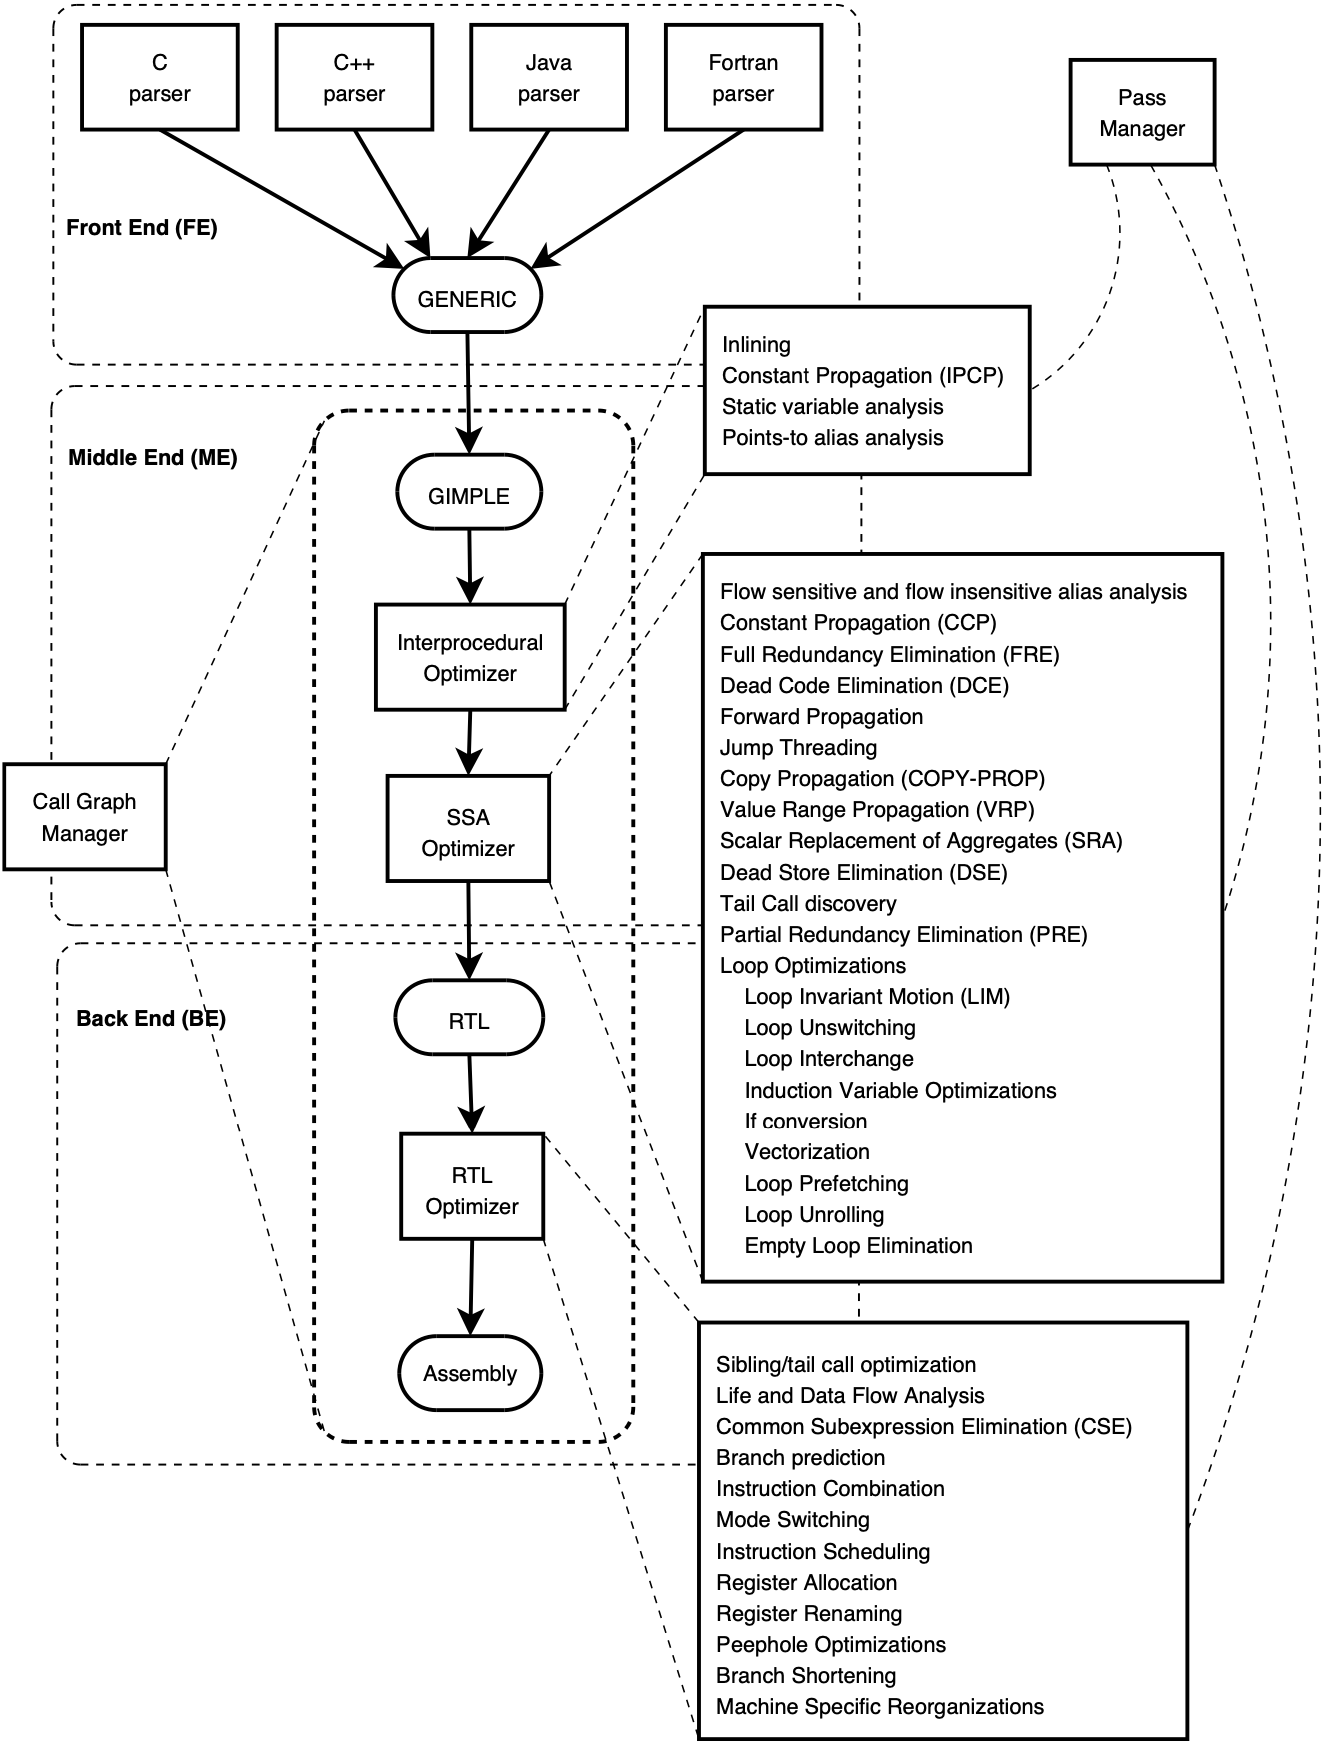
\includegraphics [width=0.95\linewidth]{pictures/GCCoverview.png}
\caption{An Overview of GCC\cite{b1}}
\label{fig1}
\end{figure}

Figure 1 shows a bird's eye view of the compiler. Notably, the various phases are orchestrated by the Call Graph and Pass managers. The call graph manager constructs a call graph for the compilation unit, determining the order in which each function should be processed. Additionally, it facilitates inter-procedural optimizations (IPO), such as inlining. On the other hand, the pass manager oversees the sequencing of individual transformations and manages pre and post cleanup actions required by each pass.

The source code is organized in three major groups: core, runtime and support. In what follows all directory names are assumed to be relative to the root directory where GCC sources live.\cite{b1}

\subsection{Optimization Level}
Typically, optimizations provided by GCC can be divided into three degrees. Some optimizations make the assembly code shorter, while others speed up the code, which potentially is enlarged.

The O1 optimization level in GCC represents a moderate level of compiler optimization designed to enhance program performance while maintaining a relatively swift compilation process. The primary focus is on applying fundamental optimizations to the code. The O1 optimization level strikes a balance between improving program performance and minimizing compilation time, making it suitable for scenarios where moderate optimization is desired without significantly impacting build times. Here are some key aspects of O1 optimization:
\begin{itemize}
	\item Unused Variable Removal:
The compiler identifies and eliminates variables that are declared but not used in the program. This helps reduce the size of the generated code.
	\item Expression Simplification:
O1 includes basic expression simplification, where the compiler aims to simplify complex expressions, potentially leading to more efficient code execution.
	\item Code Layout Optimization:
The compiler may perform basic code layout optimizations, reorganizing code sections to improve locality and potentially enhance runtime performance.
	\item Inlining of Functions:
O1 may include basic function inlining, where small functions are substituted directly into the calling code to reduce the overhead of function calls.
	\item Strength Reduction:
Basic strength reduction techniques may be applied to replace expensive operations with cheaper equivalents, optimizing arithmetic expressions for improved performance.
	\item Control Flow Optimization:
Basic control flow optimizations are employed to simplify and streamline conditional statements and loops, potentially reducing branch mispredictions.
	\item Minimization of Code Size:
While not the primary focus, O1 aims to keep the generated code relatively compact, balancing performance improvements with code size considerations.
\end{itemize}

\begin{figure}[htbp]
\centering
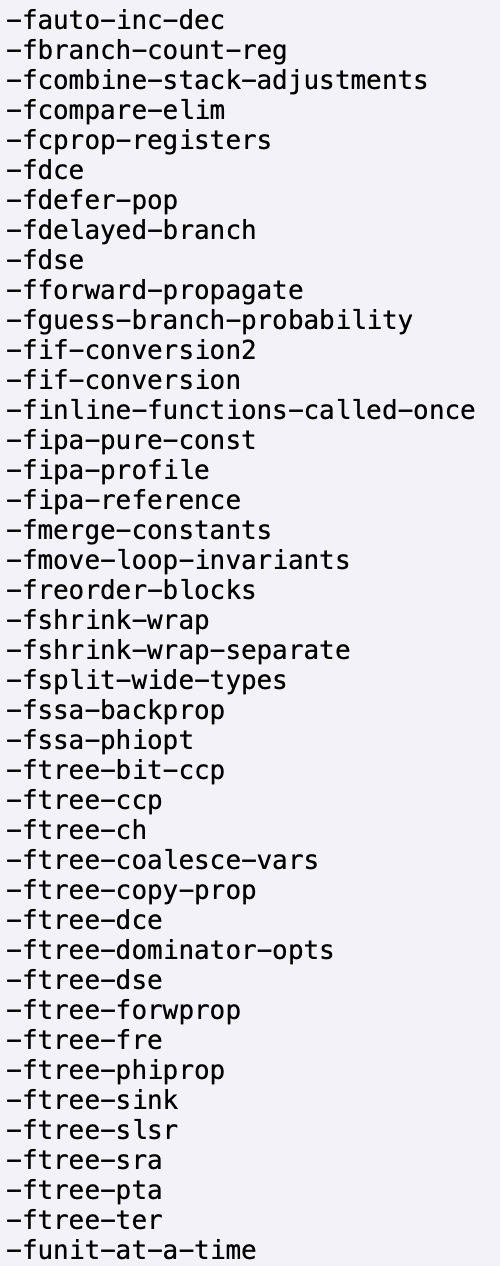
\includegraphics [width=0.4\linewidth]{pictures/o1.png}
\caption{O1 Optimization Flags\cite{b2}}
\label{fig2}
\end{figure}

The O2 optimization level in GCC encompasses a set of advanced compiler optimizations aimed at substantially improving program performance. Building upon the optimizations introduced in O1, O2 introduces more sophisticated techniques. It is characterized by a more aggressive set of optimizations, making it suitable for scenarios where achieving higher performance is a priority, even at the cost of slightly longer compilation times. Below is a detailed description, combining the objectives and impacts:
\begin{itemize}
	\item Loop Unrolling: Replicating loop bodies to reduce loop control overhead and enhance instruction-level parallelism, thereby improving execution speed.
	\item Data Flow Analysis: Analyzing the flow of data through the program facilitates a better understanding of variable relationships, leading to more effective optimizations.
	\item Cross-Module Inlining: Extending function inlining to functions defined in separate compilation units enhances opportunities for inlining across different parts of the program.
	\item Strength Reduction: Replacing expensive operations with cheaper equivalents optimizes arithmetic expressions for improved efficiency.
	\item Loop Fusion: Combining adjacent loops reduces loop overhead, improving cache locality and reducing loop control overhead.
	\item Loop Distribution: Distributing loop iterations enables better parallelization, improving the potential for parallel execution of loop iterations.
	\item Vectorization: Converting scalar operations into vector operations leverages SIMD instructions, enhancing parallelism, especially on architectures with SIMD support.
\end{itemize}

\begin{figure}[htbp]
\centering
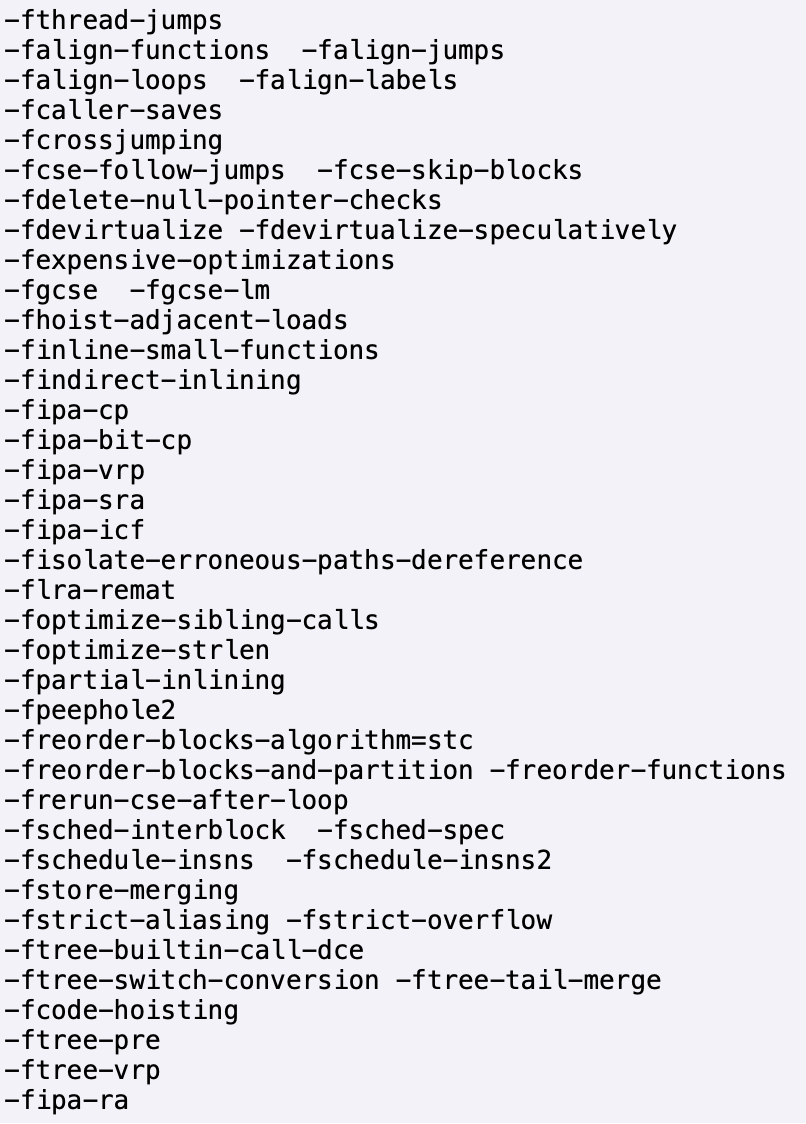
\includegraphics [width=0.7\linewidth]{pictures/o2.png}
\caption{O2 Optimization Flags\cite{b2}}
\label{fig3}
\end{figure}

The O3 optimization level in GCC represents the highest degree of compiler optimization, aimed at maximizing program performance, even if it results in longer compilation times. Building upon the optimizations introduced in O2, O3 incorporates more sophisticated and time-consuming techniques.

While the -O3 optimization level is capable of generating high-performance code, it's important to note that the resulting increase in the size of the executable can potentially have detrimental effects on its speed. Specifically, if the size of the executable surpasses the capacity of the available instruction cache, this could lead to significant performance penalties. Consequently, it might be more prudent to opt for compiling at the -O2 optimization level. This decision is driven by the intention to enhance the likelihood that the executable fits within the constraints of the instruction cache, thereby mitigating the risk of severe performance degradation.

The -Os optimization level focuses on minimizing the size of the generated executable. It aims to reduce the overall footprint of the compiled program, making it suitable for environments where compactness is a priority, such as embedded systems with limited storage.

The -Ofast optimization level is similar to -O3 but allows for more aggressive optimizations, including those that may affect mathematical precision. It prioritizes maximizing execution speed and might not be suitable for applications where strict adherence to floating-point precision is required.

To illustrate the impact of GCC compiler optimization levels, we'll use a C code example that performs numerical computations. We'll use a simple numerical integration algorithm as our case study. Below is the code without any optimizations applied:

\begin{figure}[htbp]
\centering
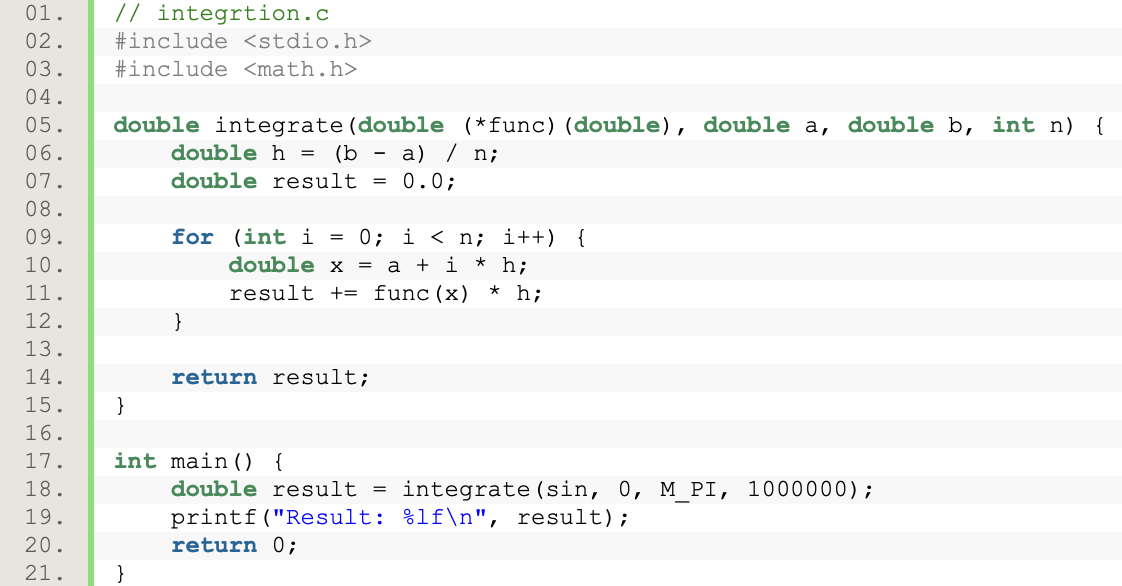
\includegraphics [width=0.9\linewidth]{pictures/gcc_sample_code.png}
\caption{C Code Example that Performs Numerical Computations\cite{b3}}
\label{fig4}
\end{figure}

Running on the same computer, the statistics are shown in Table 1. The `Real' time is the actual wall-clock time it took to execute the program. The `User' time represents the CPU time consumed by the program. The `Sys' time indicates system-related CPU time.\cite{b3}

\begin{table}
	\caption{Running Time\cite{b3}}
	\begin{center}
		\begin{tabular}{c c c c c c}
			\toprule
			Optimization &default&O2&O3&Os&Ofast\\
			\hline
			Real & 0.064s & 0.041s & 0.058s & 0.016s & 0.067s\\
			User & 0.064s & 0.041s & 0.058s & 0.015s & 0.066s\\
			Sys  & 0.001s & 0.001s & 0.001s & 0.001s & 0.001s\\
			\bottomrule
		\end{tabular}
	\end{center}
\end{table}

Specifying the target architecture can also yield meaningful benefits. The -march option of gcc allows the CPU type to be specified. The default architecture is i386. GCC runs on all other i386/x86 architectures, but it can result in degraded performance on more recent processors. Let's now look at an example of how performance can be improved by focusing on the actual target. Build a simple test application that performs a bubble sort over $10000$ elements. The elements in the array have been reversed to force the worst-case scenario.\cite{b4}

\begin{figure}[htbp]
\centering
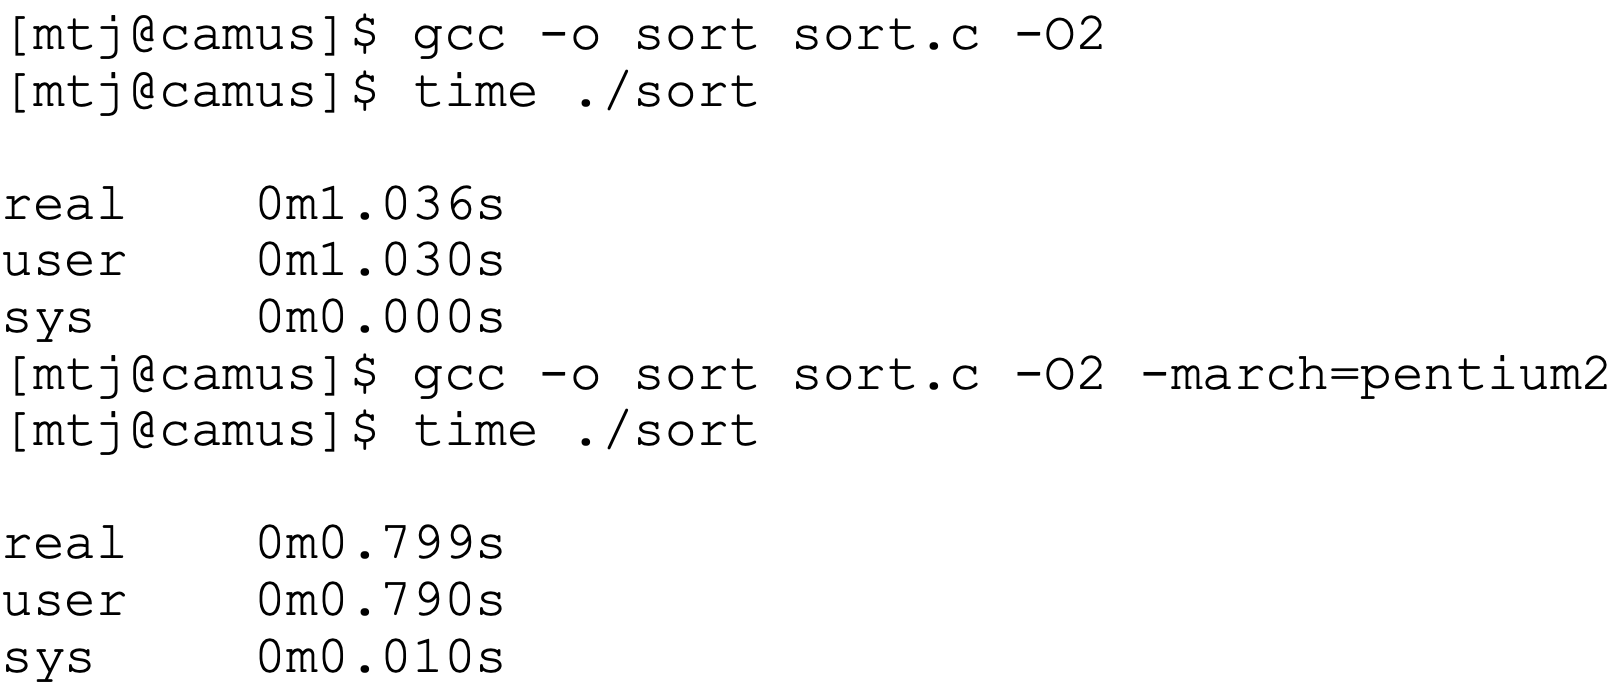
\includegraphics [width=0.85\linewidth]{pictures/GCCarchi.png}
\caption{Effects of Architecture Specification on a Simple Application\cite{b4}}
\label{fig5}
\end{figure}

By specifying the architecture, in this case a 633MHz Celeron, the compiler can generate instructions for the particular target as well as enable other optimizations available only to that target. As shown in Figure 5, by specifying the architecture we see a time benefit of 237ms (23\% improvement). Although it shows an improvement in speed, the drawback is that the image is slightly larger. Using the size command, we can identify the sizes of the various sections of the image, which is shown in Figure 6.\cite{b4}

\begin{figure}[htbp]
\centering
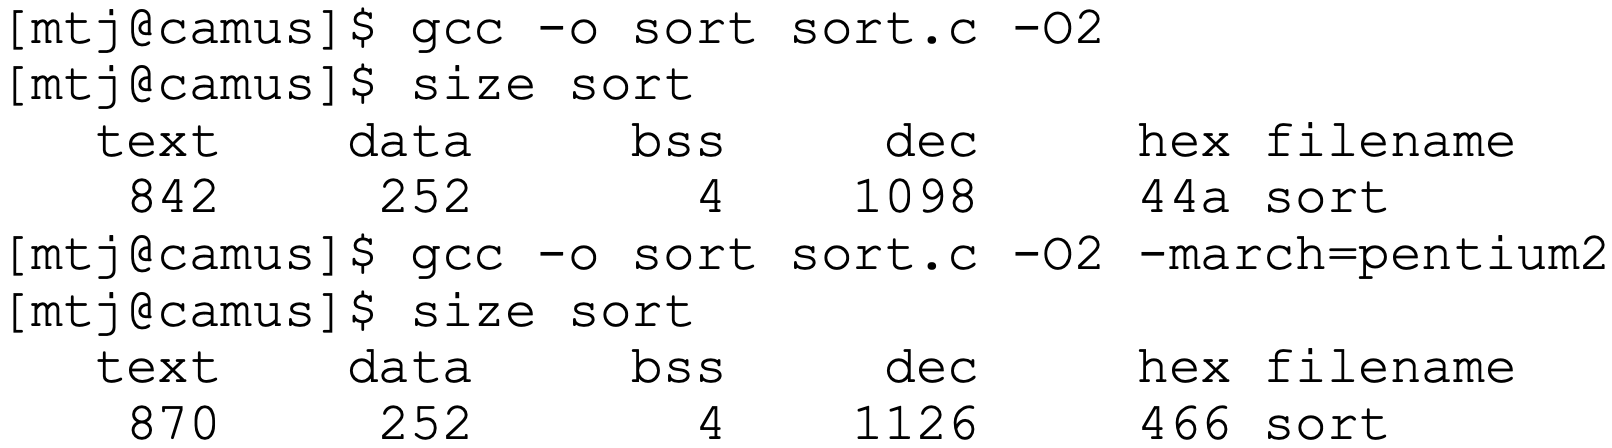
\includegraphics [width=0.85\linewidth]{pictures/GCCsize.png}
\caption{Size Change of the Application\cite{b4}}
\label{fig6}
\end{figure}

Here the instruction size (text section) of the image increased by 28 bytes. But in this example, it's a small price to pay for the speed benefit.\cite{b4}

In conclusion, optimizing your code with GCC is not just a luxury but a necessity in today's demanding software landscape. A profound understanding of the diverse optimization levels and their judicious application can elevate your code to the status of an efficient, high-performing masterpiece.

However, a word of caution is essential. Optimization is akin to a double-edged sword. While it has the potential to deliver remarkable performance gains, it should not come at the expense of the readability and maintainability of your code. Striking the delicate balance between optimization and code quality is an art that every developer must master.

\subsection{Vectorization}

Vectorization in GCC refers to the process of transforming scalar operations within code into vector operations, a technique particularly pertinent to SIMD (Single Instruction, Multiple Data) architectures where a single instruction can concurrently operate on multiple data elements.

The objective of vectorization is to enhance parallelism and harness the capabilities of contemporary processors equipped with vector units. These vector units facilitate the simultaneous execution of a single instruction on multiple data elements, thereby amplifying throughput and overall performance.

In Figure 7, the compiler on the left is capable of computing only one pair of scalar multiplications at a time. Consequently, the multiplication of four pairs of numbers requires four separate operations. Conversely, the compiler on the right possesses the capability to concurrently process four numbers, enabling the completion of the multiplication of four pairs of numbers in a single operation.

\begin{figure}[htbp]
\centering
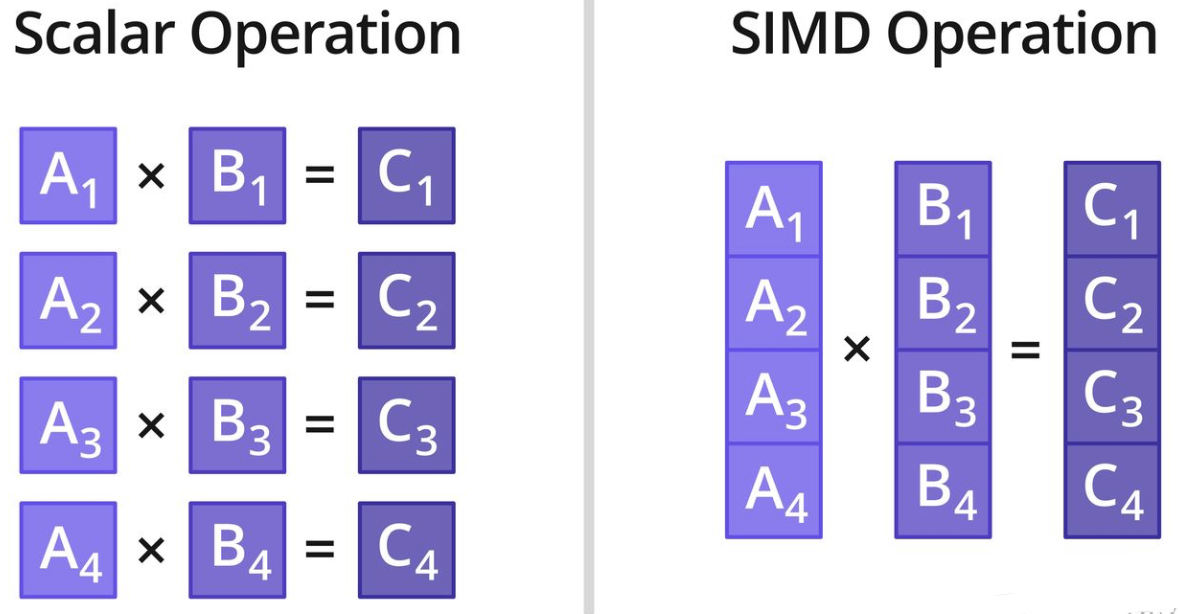
\includegraphics [width=0.8\linewidth]{pictures/SIMD.png}
\caption{A comparison between scalar and SIMD operation\cite{b5}}
\label{fig7}
\end{figure}

In modern computing, SIMD processing units or GPUs are primarily employed for vector processing. High-end CPUs commonly integrate specialized instruction sets for SIMD operations, such as Intel's SSE and AVX. The SIMD processing capability of CPUs operates in a parallel fashion within a single core. The parallel paradigm in multicore processing is referred to as MIMD (multiple instruction multiple data). The distinction lies in SIMD's execution in a lockstep manner, where all ALU units share a single program counter (PC). In contrast, MIMD involves independent execution across cores, each with its own PC.

In GCC, using vector instructions through built-in functions is available. On some targets, the instruction set contains SIMD vector instructions which operate on multiple values contained in one large register at the same time.\cite{b6}

Assuming our SIMD processor can handle $4$ double numbers at once, take an addition of two arrays as an example in Figure 8. Inside the loop in line 14, it loads four single-precision floating-point values from the array $a$ into a Neon vector $va$. Then it adds the loaded vector $va$ element-wise to the cumulative sum vector $vsum$. It accumulates the sum as the loop progresses. After the loop, it uses Neon intrinsics to perform pairwise addition on the lower and higher lanes of the cumulative sum vector $vsum$, resulting in a 2-element vector $sum_lane$. Finally it completes the reduction by adding the two elements of the 2-element vector $sum_lane$. The result is a single-precision floating-point value representing the sum of the vectorized elements.

\begin{figure}[htbp]
\centering
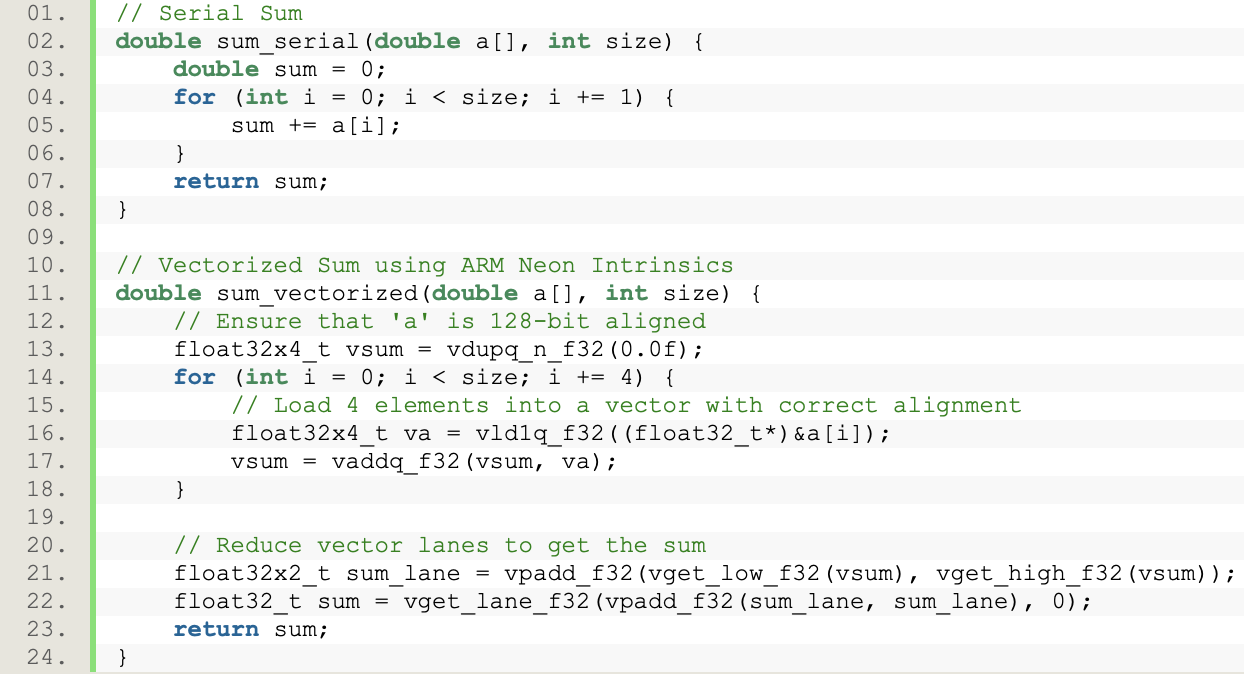
\includegraphics [width=0.95\linewidth]{pictures/SIMD_code.png}
\caption{SIMD Code Example}
\label{fig8}
\end{figure}

When the array size is $100000000$, the serial time and vectorized time is $0.3656$ seconds and $0.1772$ seconds (Apple M2), respectively, which indicates a crucial speedup.

In the context of parallelized numerical accumulation, it is essential to recognize that the order of summation may change due to parallel processing. To achieve parallelism, associativity, the property that allows rearrangement of operands without altering the result (e.g., $a+b+c+d=(a+b)+(c+d))$, becomes crucial. This property ensures that parallel addition remains consistent even with a different summation order.

However, when dealing with floating-point operations involving multiplication or addition, achieving strict associativity can be challenging. Floating-point arithmetic, subject to rounding errors, may not strictly adhere to associativity, especially when parallelized. Consequently, to facilitate parallel floating-point operations, specialized compiler options such as `--ffast-math' in GCC are often employed. These options relax strict adherence to IEEE standard compliance and allow for more aggressive optimizations.

Maintaining numerical stability in the face of reordering operations for parallelism is a fundamental concern. Rounding errors, inherent in floating-point calculations, can accumulate differently depending on the order of operations. Achieving both parallelism and numerical stability requires a delicate balance. The use of appropriate compiler flags, careful algorithm design, and consideration of numerical stability principles are essential in minimizing the impact of rounding errors and ensuring reliable parallel computations.

Now take one more complex example into consideration. That is matrix multiplication, which is widely used, forming the foundational logic for numerous algorithms. This paper will compare the time consumption of different approaches in matrix operations, with a focus on exploring the efficacy of O3 optimization and elucidating the methodologies potentially employed by O3 optimization.

Sample codes are stored in MatrixMultiplication folder. In Matrix.h we define a matrix, simultaneously, in Matrix.c we define how it works. Suppose we have two matrices $mtx1$ and $mtx2$, and then set $ans$ equal to $mtx1 \times mtx2$.

Just follow the principle of matrix multiplication we can write a plain method, which is shown in Figure 9.

\begin{figure}[htbp]
\centering
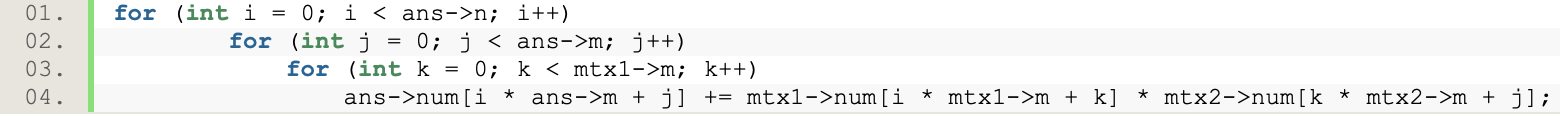
\includegraphics [width=0.95\linewidth]{pictures/plain.png}
\caption{Matrix Multiplication Plain Method}
\label{fig9}
\end{figure}

Optimizing cache utilization is critical for enhancing computational efficiency. One effective strategy involves manipulating the loop order to improve cache hit rates, specifically by employing a technique known as loop interchange. By employing loop interchange, the order of traversal is rearranged, typically from $ijk$ to $ikj$.

When computing each element of the matrix \( C = A \times B \) using the Plain Method, a vector dot product is performed between the rows of matrix \( A \) and the columns of matrix \( B \). As matrices are stored row-wise, accessing individual elements of the corresponding row in matrix \( A \) results in contiguous memory access. However, for matrix \( B \), which requires column-wise computation, accessing current and subsequent positions in memory is non-contiguous. Upon completion of the computation, matrix \( B \) incurs \( n \) jumps in memory access, resulting in \( n^3 \) jumps after \( n^2 \) computations.

By altering the loop order from \( ijk \) to \( ikj \), the program performs row-wise computations for the elements of \( C \). While computing the first element in a row, access is made to the first element in the corresponding row of \( A \) and the first element in the corresponding column of \( B \). When calculating the subsequent element, the \( B \) pointer increments by one position while the \( A \) pointer remains stationary. After completing the calculation for all elements in that row of \( C \), the \( A \) pointer moves one position to the right. Consequently, each computation of an element in \( C \) incurs only one jump, resulting in a total of \( n^2 \) jumps after \( n^2 \) computations.

Notably, when transitioning to the next row after accessing the current row, there is no jump if using a one-dimensional array for storage, whereas one jump occurs if using a two-dimensional array.

The relationship between the number of jumps and loop order, as well as storage format, is summarized in Table II. Furthermore, the inner loop can be vectorized, utilizing hardware-provided fused multiply-add (FMA) operations, with subsequent unrolling. If compiler optimizations are enabled, manual unrolling becomes unnecessary.

\begin{table}
	\caption{Number of Jumps}
	\begin{center}
		\begin{tabular}{c c c}
			\toprule
			Order &One-dimensional array&Two-dimensional array\\
			\hline
			 $ikj$  &    $n^2$    &    $2n^2+n$  \\  
 $kij$  &   $2n^2$      &   $3n^2$     \\
 $jik$ & $n^{3}+n^2+n$  & $n^3+2n^2$   \\
 $ijk$ &  $n^3+n^2-n$  & $n^{3}+n^2+n$ \\
 $kji$  &   $2n^3$    &    $2n^3+n$    \\
 $jki$ &  $2n^3+n^2$  &   $2n^3+n^2$   \\
			\bottomrule
		\end{tabular}
	\end{center}
\end{table}

Additionally, SIMD optimization can be employed. During each computation, a \(4 \times 4\) small block is calculated by extracting \(4\) rows from matrix \(A\) and \(4\) columns from matrix \(B\). Each row and column are reused \(4\) times in this process, with all data reuse occurring in the cache, effectively reducing the number of memory accesses. To ensure contiguous reading for each row, the corresponding data is packed into \(4\) one-dimensional arrays after computing \(4\) rows, and these arrays are repacked for the next \(4\) rows after completing all terms in the product related to these data.

If the matrices are sufficiently large, and \(4\) rows or columns cannot fit into the cache, matrix \(A\) can be divided into row vectors, and matrix \(B\) into column vectors. Finally, SSE instructions are utilized to accelerate the multiplication operation. If AVX2.0 is employed, processing \(4\) double-precision floating-point numbers simultaneously is possible, thereby doubling the efficiency.

The time costed by different method is shown in Table III (AMD R5-5500U). In the `MatrixMultiplication' directory, execute `Test.cpp' to obtain the corresponding output. Note that the runtime performance during execution may be influenced by factors such as CPU architecture and capabilities, operating system, available system memory, and other related considerations.

\begin{table}
	\caption{Time Costed by Different Method}
	\begin{center}
		\begin{tabular}{c c c c c}
			\toprule
			$N$ &Plain&Loop interchange & O3 & SIMD\\
			\hline
			$16$ & $0$ms & $0$ms & $0$ms & $0$ms\\
			$128$& $3$ms& $1$ms& $0$ms& $0$ms\\
			$256$& $1802$ms& $555$ms& $627$ms& $95$ms\\
			$2000$& $16049$ms& $4347$ms& $4164$ms& $507$ms\\
			\bottomrule
		\end{tabular}
	\end{center}
\end{table}

From Table III, it can be observed that the runtime after O3 optimization and after swapping loop order are relatively close, and both are significantly higher than the runtime after SIMD optimization. This suggests that O3 optimization may alter the loop order and does not inherently provide SIMD optimization.

In conclusion, GCC provides robust support for automatic vectorization, enabling the compiler to detect and transform segments of code suitable for vectorization at compile time. This automatic vectorization is performed without explicit directives from the programmer, relying on the compiler's analysis of data dependencies and loop structures to identify vectorizable portions. In fields dealing with large datasets and scientific computing, vectorization plays a crucial role within the GCC compiler.

\subsection{Back-end Optimization Analysis}

Register Transfer Language (RTL) is a crucial intermediate representation in the context of compiler construction, serving as a pivotal bridge between high-level source code and low-level machine code within the framework of GCC. The RTL generation, optimization, and assembly code generation processes constitute an intricate series of stages aimed at transforming abstract program structures into efficient machine-executable instructions.

The RTL generation process involves the translation of the abstract syntax tree (AST) derived from the high-level source code into a hardware-oriented, register-transfer-based representation. This step captures the essential data and control flow aspects of the program, representing them in terms of RTL operations and their associated operands. This intermediate form serves as a foundation for subsequent analyses and transformations.

RTL optimization encompasses a suite of techniques geared toward enhancing the performance of the generated code. This involves a myriad of low-level optimizations such as register allocation, instruction scheduling, and dead code elimination. Register allocation seeks to judiciously assign program variables to processor registers, minimizing memory accesses and improving overall execution speed. Instruction scheduling aims to reorder operations to exploit parallelism and reduce pipeline stalls. Additionally, dead code elimination identifies and removes code segments that contribute no discernible impact on program output.

Subsequent to RTL optimization, the compiler proceeds to the generation of assembly code tailored to the target architecture. This involves mapping RTL operations and operands to specific machine instructions, considering the intricacies of the underlying hardware. The assembly code generated at this stage serves as the final output that can be further processed by an assembler to produce machine code executable on the target platform.

The processes of RTL generation, optimization and assembly code generation, should be guided by machine description. The machine descriptions are composed of three files: target machine-description macro definitions file (target.h), machine-description functions support file (target.c) and target machine descriptions file (target.md).\cite{b7}

These descriptions play a pivotal role in the backend stages of the compiler, particularly during the code generation phase. Compiler utilization of machine descriptions ensures the generation of assembly code congruent with the target machine architecture. These descriptions not only furnish the compiler with the requisite information for the production of correct code but also endow the optimizer with insights, facilitating the adept utilization of the target machine's features to enhance code performance.

\begin{figure}[htbp]
\centering
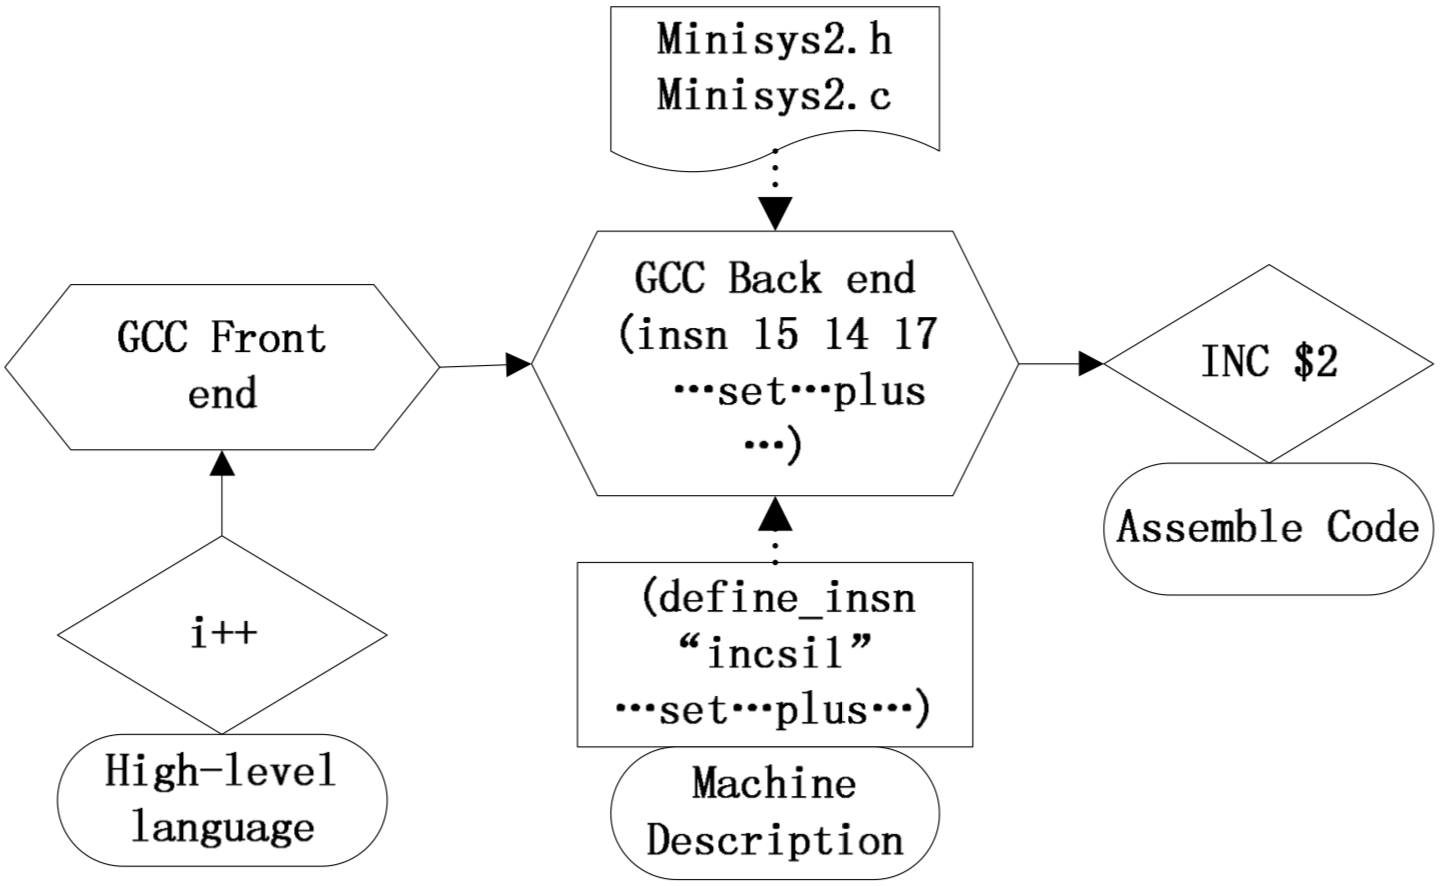
\includegraphics [width=0.95\linewidth]{pictures/i++.png}
\caption{Example Code `i++' Compilation Process\cite{b7}}
\label{fig10}
\end{figure}

It deserves to be mentioned that the efficiency of complier should be taken into full account in the porting process. As the pattern of each instruction is matched in order, the more instruction patterns there are, the more slowly the compiling system will be. It is better to combine the similar instructions to one instruction pattern to obtain higher complier efficiency. The priority of instruction matching should be paid attention to at the same time. Take a simple C language sentence `i++' as an example and set the target machine as Minisys2. The result of matching can be `INC \$2', as well as the mode of `add \$2, \$3, 1'. The process of matching `target.md' file is carried out through the order from top to bottom in GCC, so `INC' instruction pattern should be put in the front of `add' instruction pattern in order to test the newly increased “INC” instruction.\cite{b7}

In summation, machine descriptions serve as crucial metadata in the compiler domain, delineating how the compiler interfaces with a specific target architecture, thereby enabling the production of accurate and efficient machine code.

\subsection{Summary of GCC}

GCC plays a pivotal role in the entire process of translating source code into target machine executable code. Its impact extends across critical facets of software development.

The primary function of GCC lies in the transformation of source code, authored in high-level programming languages such as C and C++, into executable code for the target machine. It accommodates various target architectures, enabling developers to create and execute programs on diverse platforms.

As an open-source and widely adopted compiler, GCC has exerted a profound influence on the entire software ecosystem. It affords developers the capability for cross-platform development, fostering software portability. Furthermore, the existence of GCC has propelled advancements in compiler technology, serving as a template for numerous other compiler projects.

GCC incorporates a potent optimizer capable of enhancing the performance of the generated target code during the compilation process. Optimization spans various dimensions, encompassing, but not limited to, constant folding, register allocation, instruction scheduling, and loop optimization. Through these optimization techniques, GCC generates machine code that is not only more efficient but also aligns closely with the underlying hardware capabilities.

\section{Distinction of Clang/LLVM}

LLVM (Low Level Virtual Machine) is a compiler infrastructure project designed to provide a flexible and extensible compiler framework. It comprises a suite of general-purpose compiler tools, including frontends responsible for source code parsing, optimizers tasked with enhancing intermediate code, and backends responsible for generating target code. The design of LLVM emphasizes modularity and reusability, making it a preferred framework for compiler implementations and optimization tools across various programming languages.

Clang is an open-source, cross-platform compiler for the C, C++, Objective-C, and Objective-C++ programming languages. It is part of the LLVM project and is designed to offer a high-performance, modular, and extensible compiler frontend. The design of Clang emphasizes code clarity and readability, making it a preferred compiler for many developers and projects.

\subsection{Introduction}

Figure 11 illustrates the basic architecture of Clang/LLVM. Initially, the frontend for LLVM was GCC. Subsequently, Apple aspired to develop its own Clang to replace GCC. Moreover, it is possible to develop custom frontends, which, when combined with the LLVM backend, enable the creation of compilers for custom programming languages.

\begin{figure}[htbp]
\centering
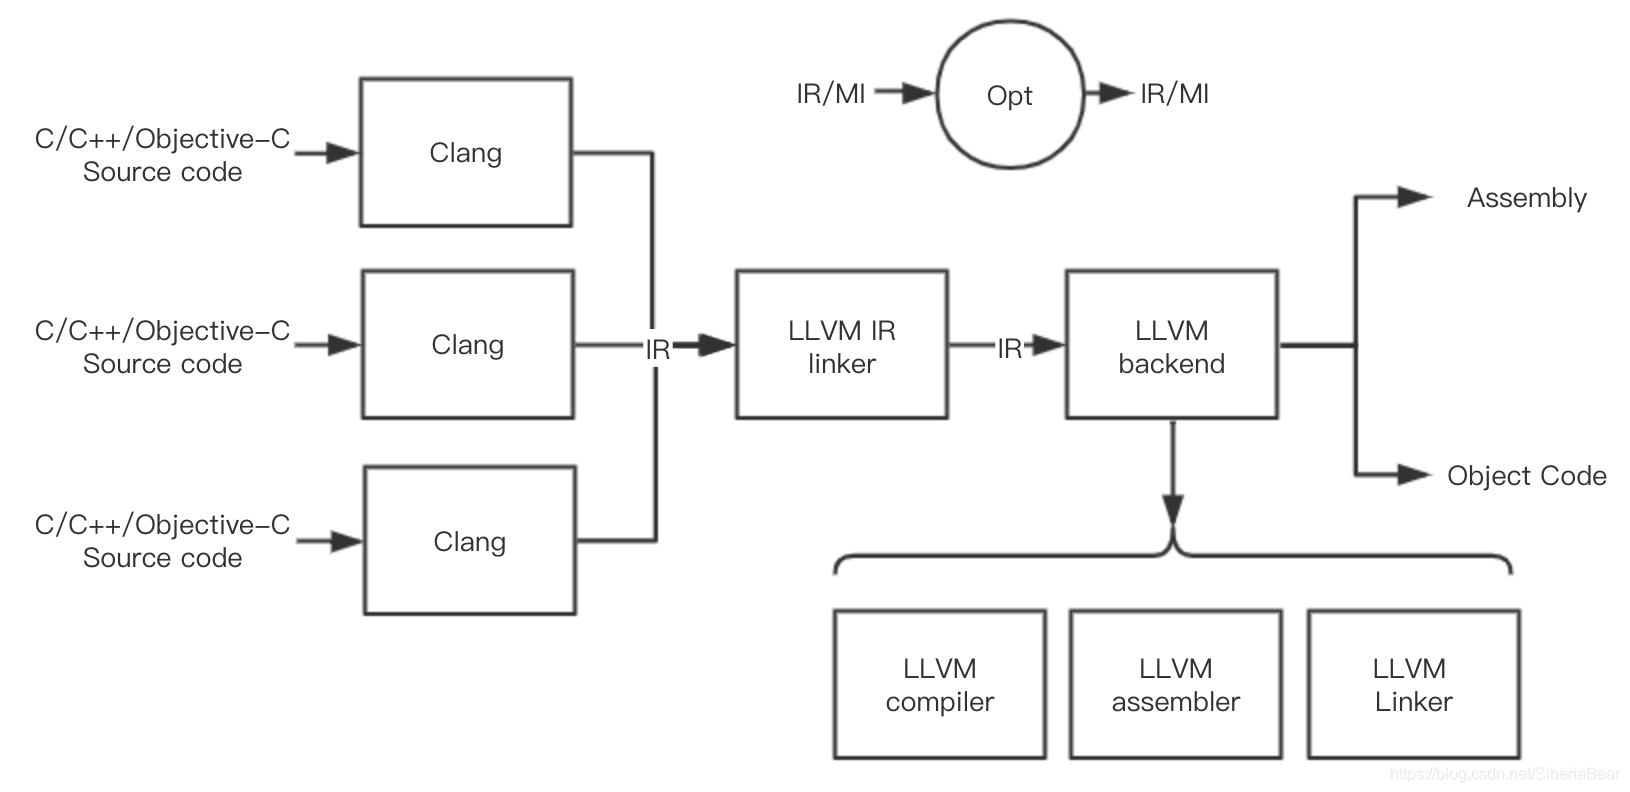
\includegraphics [width=1\linewidth]{pictures/ClangLLVMoverview.png}
\caption{Architecture of Clang/LLVM\cite{b8}}
\label{fig11}
\end{figure}

In LLVM, Intermediate Representation (IR) exists in three forms.

The first is a human-readable IR, akin to assembly code, albeit positioned between high-level languages and assembly. This representation is designed for human consumption, and its disk file suffix is .ll.

The second form is an unreadable binary IR, known as bitcode, with a disk file suffix of .bc.

The third representation is a memory format, exclusively stored in memory, devoid of any file format or suffix. This format contributes to LLVM's swift compilation, distinct from GCC, which generates intermediate process files at the conclusion of each stage. LLVM's intermediate data at various compilation stages is in the form of this third representation of IR.

In LLVM IR, a compilation unit (i.e., a .c file) represents a Module. Within a Module, there are Global Values, primarily comprising Global Variables and Functions. A Function encompasses Basic Blocks, and each Basic Block contains instructions, such as "add". Therefore, the hierarchical relationship can be conceptualized as Module - Function - Basic Block - Instructions. Some APIs of LLVM IR might be referred like Figure 12.

\begin{figure}[htbp]
\centering
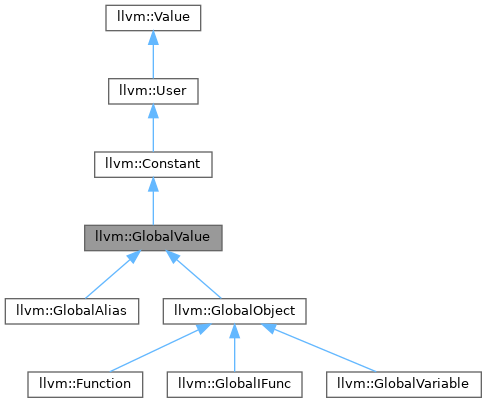
\includegraphics [width=0.95\linewidth]{pictures/LLVMInheritanceDiagram.png}
\caption{Inheritance Diagram for llvm::GlobalValue\cite{b10}}
\label{fig12}
\end{figure}

All three representations are entirely equivalent. While Clang/LLVM tools do not generate these files by default (typically unnecessary for non-compiler developers), they can be specified using parameters in the toolchain. Conversion between the first two file types can be facilitated using llvm-as and llvm-dis.

Notably, there is an LLVM IR linker in the process, distinct from the linker in GCC. To achieve link-time optimization, LLVM, after generating IR for individual code units in the frontend (Clang), links the entire project's IR while concurrently performing link-time optimizations.

The LLVM backend constitutes the genuine backend of LLVM, also referred to as the LLVM core. It encompasses compilation, assembly, and linking processes, ultimately producing assembly files or target code. It is important to differentiate the LLVM compiler here from the compiler in GCC; in LLVM, the LLVM compiler exclusively compiles LLVM IR.

\begin{figure}[htbp]
\centering
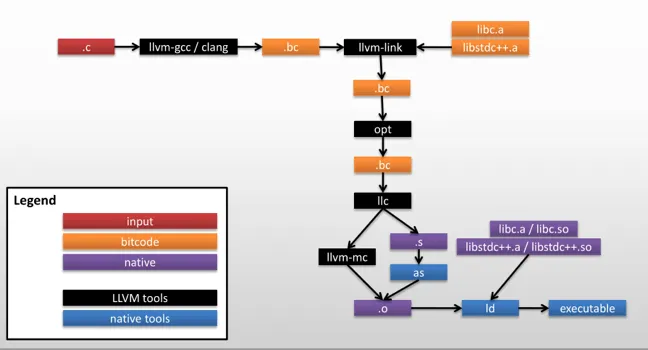
\includegraphics [width=0.95\linewidth]{pictures/ClangProcedure.png}
\caption{Procedure of Clang/LLVM\cite{b9}}
\label{fig13}
\end{figure}

Figure 13 illustrates the procedure a C code will go through in Clang/LLVM. Firstly, we have C source code program files, which then undergo the Clang frontend (or the deprecated llvm-gcc frontend, used prior to the advent of Clang, capable of generating LLVM IR). Subsequently, LLVM IR is produced. In this context, LLVM IR is identified by the .bc extension, representing a serialized data format utilized for storage on disk. However, LLVM IR also boasts another remarkable feature in the form of a human-readable format, typically denoted by the .ll extension. Figure 14 is an example of the human-readable format for a simple C language Hello World program:

\begin{figure}[htbp]
\centering
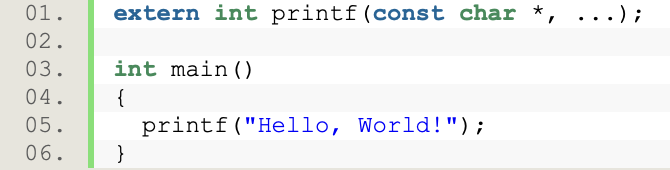
\includegraphics [width=0.95\linewidth]{pictures/helloworld.png}
\caption{Hello-world Human-readable Format}
\label{fig14}
\end{figure}

Use `clang a.c -S -emit-llvm' to generate .ll file, which is shown in Figure 15. It's useful to obtain information of more instructions referring to LLVM Language Reference Manual\cite{b11}.

\begin{figure}[htbp]
\centering
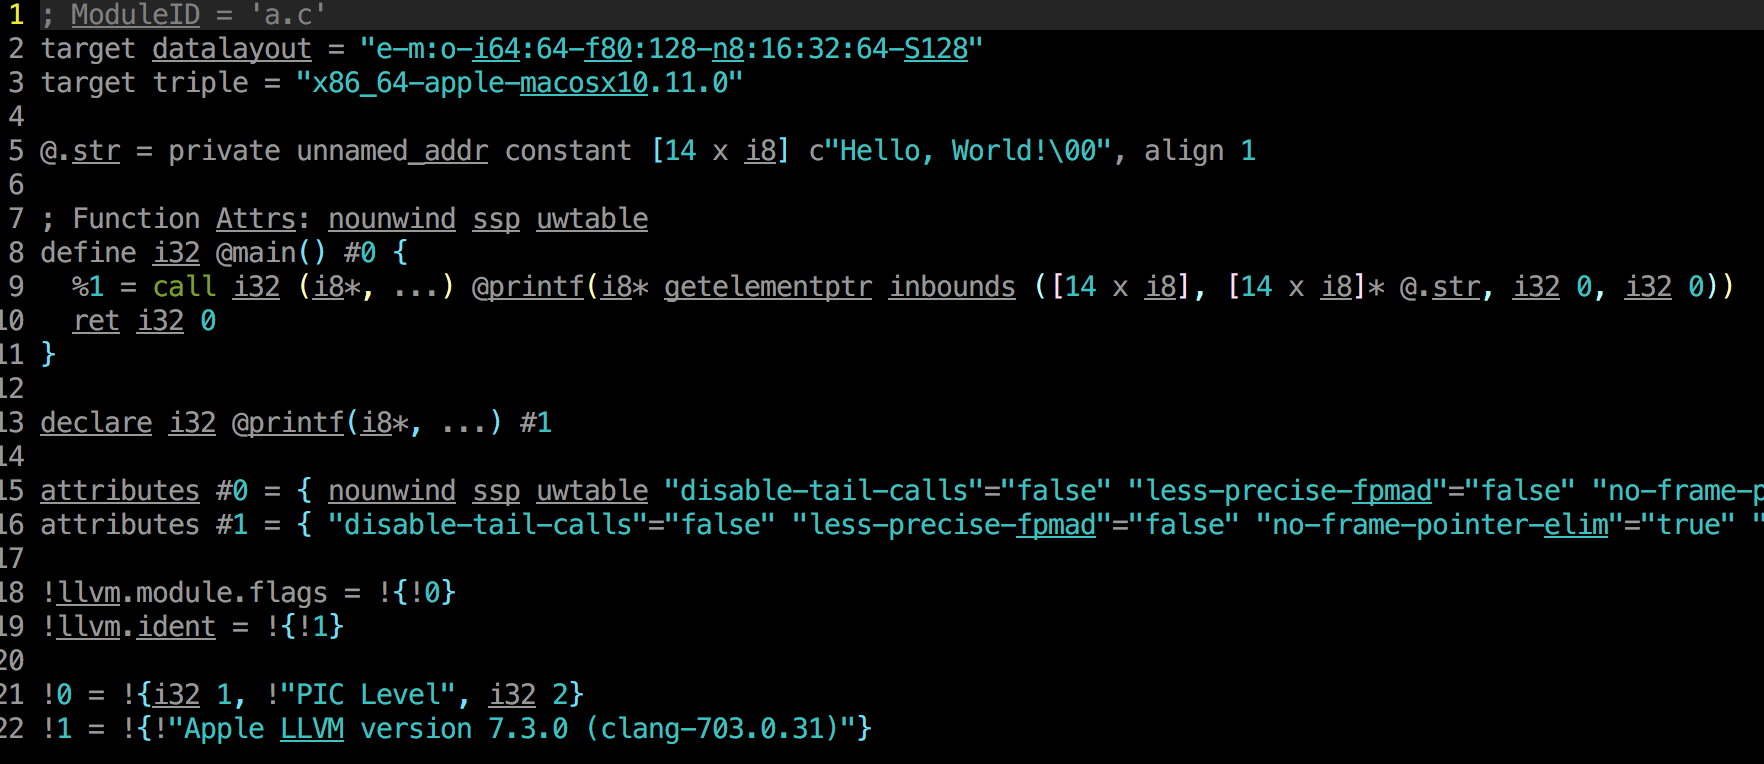
\includegraphics [width=0.95\linewidth]{pictures/llFile.png}
\caption{Content of .ll File\cite{b9}}
\label{fig15}
\end{figure}

After the completion of the generation of the .bc file, if optimizations such as O2 are applied, there is an additional optimization phase known as unit-level optimization. This phase encompasses approximately 40 optimization passes, including dead code elimination, inlining, and others. Despite the optimizations, the output remains in the .bc file format. Subsequently, the process proceeds to the llvm-link stage. During the llvm-link stage, the primary objective is to merge multiple .bc files into a single .bc file while simultaneously performing link-time optimizations, which will be explained later.

After the llvm-link stage, we obtain a new .bc file, prompting another round of optimization. This is necessary because llvm-link might introduce structural changes to the IR, potentially making it more amenable to optimization. Subsequent to this step, the final optimized .bc file is obtained, marking the formal entry into the code generation phase.

In Figure 13, only llc, representing the path for machine code generation, is illustrated. However, LLVM also supports an additional process, namely lli, which involves interpreting the LLVM IR. Although this paper won't delve into this here, the focus remains on machine code generation. The role of llc is to compile LLVM IR into an assembly file (.s). Roughly, LLVM IR can be treated as a programming language, and after passing through the llc compiler, an assembly file is produced. Analogous to the generation of LLVM IR from a C program through Clang, the generation of an assembly file is achieved.

Following the creation of the assembly file, the system assembler, such as GNU's as, is invoked to generate the object file (.o). Attentive readers might notice another path involving llvm-mc, a direct route to generating the object file. However, this path is not universally followed on all platforms, and the key lies in LLVM's integrated assembler, denoted by `-fintegrated-as'. Using the integrated assembler, one can go from MCLowering to MCInst and then employ MCStreamers to generate the .o directly, or alternatively, generate the .s file. \cite{b9}

Once the .o file has been generated, the remaining process is relatively straightforward. It involves the linker linking relevant libraries and combining them with the object file to produce the executable file with extensions like .out or .exe.

In summary, the Clang/LLVM workflow initiates from source code, undergoes multiple stages of transformation, optimization, and linking, ultimately yielding an executable file. The modular and extensible nature of this workflow positions it as a robust tool widely utilized in compiler and toolchain development.

\subsection{Clang Driver}

The driver of a compiler is a program that controls and coordinates the entire compilation process. It receives compilation options and source code files provided by the user, and is responsible for invoking various components of the compiler, such as the preprocessor, compiler proper, assembler, and linker, to generate the final executable or object file. The compiler's driver plays an organizational and managerial role during the compilation process, ensuring that each compilation phase is invoked in the correct order with the appropriate parameters.

In practical engineering, the term `driver' pertains to concrete issues rather than theoretical aspects of compilation. Questions such as how to set compiler options, what interfaces to provide to users, and how to utilize these interfaces are considerations in the development of compiler products, falling outside the typical scope covered in compiler theory textbooks.

However, the `driver' constitutes a crucial component in actual compilers, serving as a direct interface for programmer-users and significantly influencing user experience. For instance, when utilizing the GCC compiler and configuring numerous compiler options, if there is a need to port it to other platforms or support additional compilers, it often requires adjustments to compiler options rather than modifications to your code. For example, using `-std=c++11' to enable C++11 features, while on IBM's compiler on AIX, the corresponding option is `-qlanglvl=extended0x', and Microsoft's MSVC on Windows does not recognize the `-std=c++11 option.

Figure 16 shows how Clang driver works. The orange portion in this diagram not only symbolizes the mentioned input/output in the top-left corner of the image but also represents the specific data structures within the Clang Driver, such as the ArgList as you observed. The green section not only stands for Driver Functions but also signifies the concrete execution flow within the Driver. The blue-purple segment encompasses some significant auxiliary classes.

\begin{figure}[htbp]
\centering
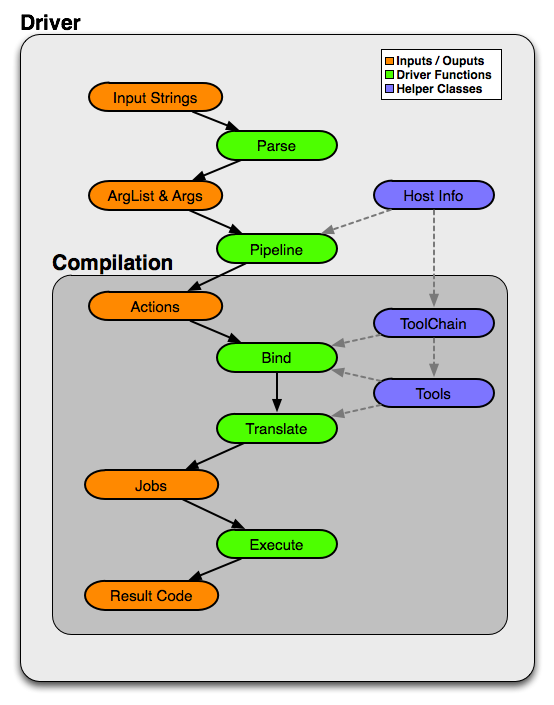
\includegraphics [width=0.9\linewidth]{pictures/ClangDriver.png}
\caption{Clang Driver\cite{b12}}
\label{fig16}
\end{figure}

Firstly, the role of Parse is option parsing. It is responsible for parsing the command-line options provided by the user into individual parameters and placing them into instances of the Arg class. Suppose we have a file named `a.c' containing only one line, which is `int main()\{\}'. In terminal, as an example, use `clang -\#\#\# a.c -I/CS323/2023F' to compile it. The result is shown in Figure 17.

\begin{figure}[htbp]
\centering
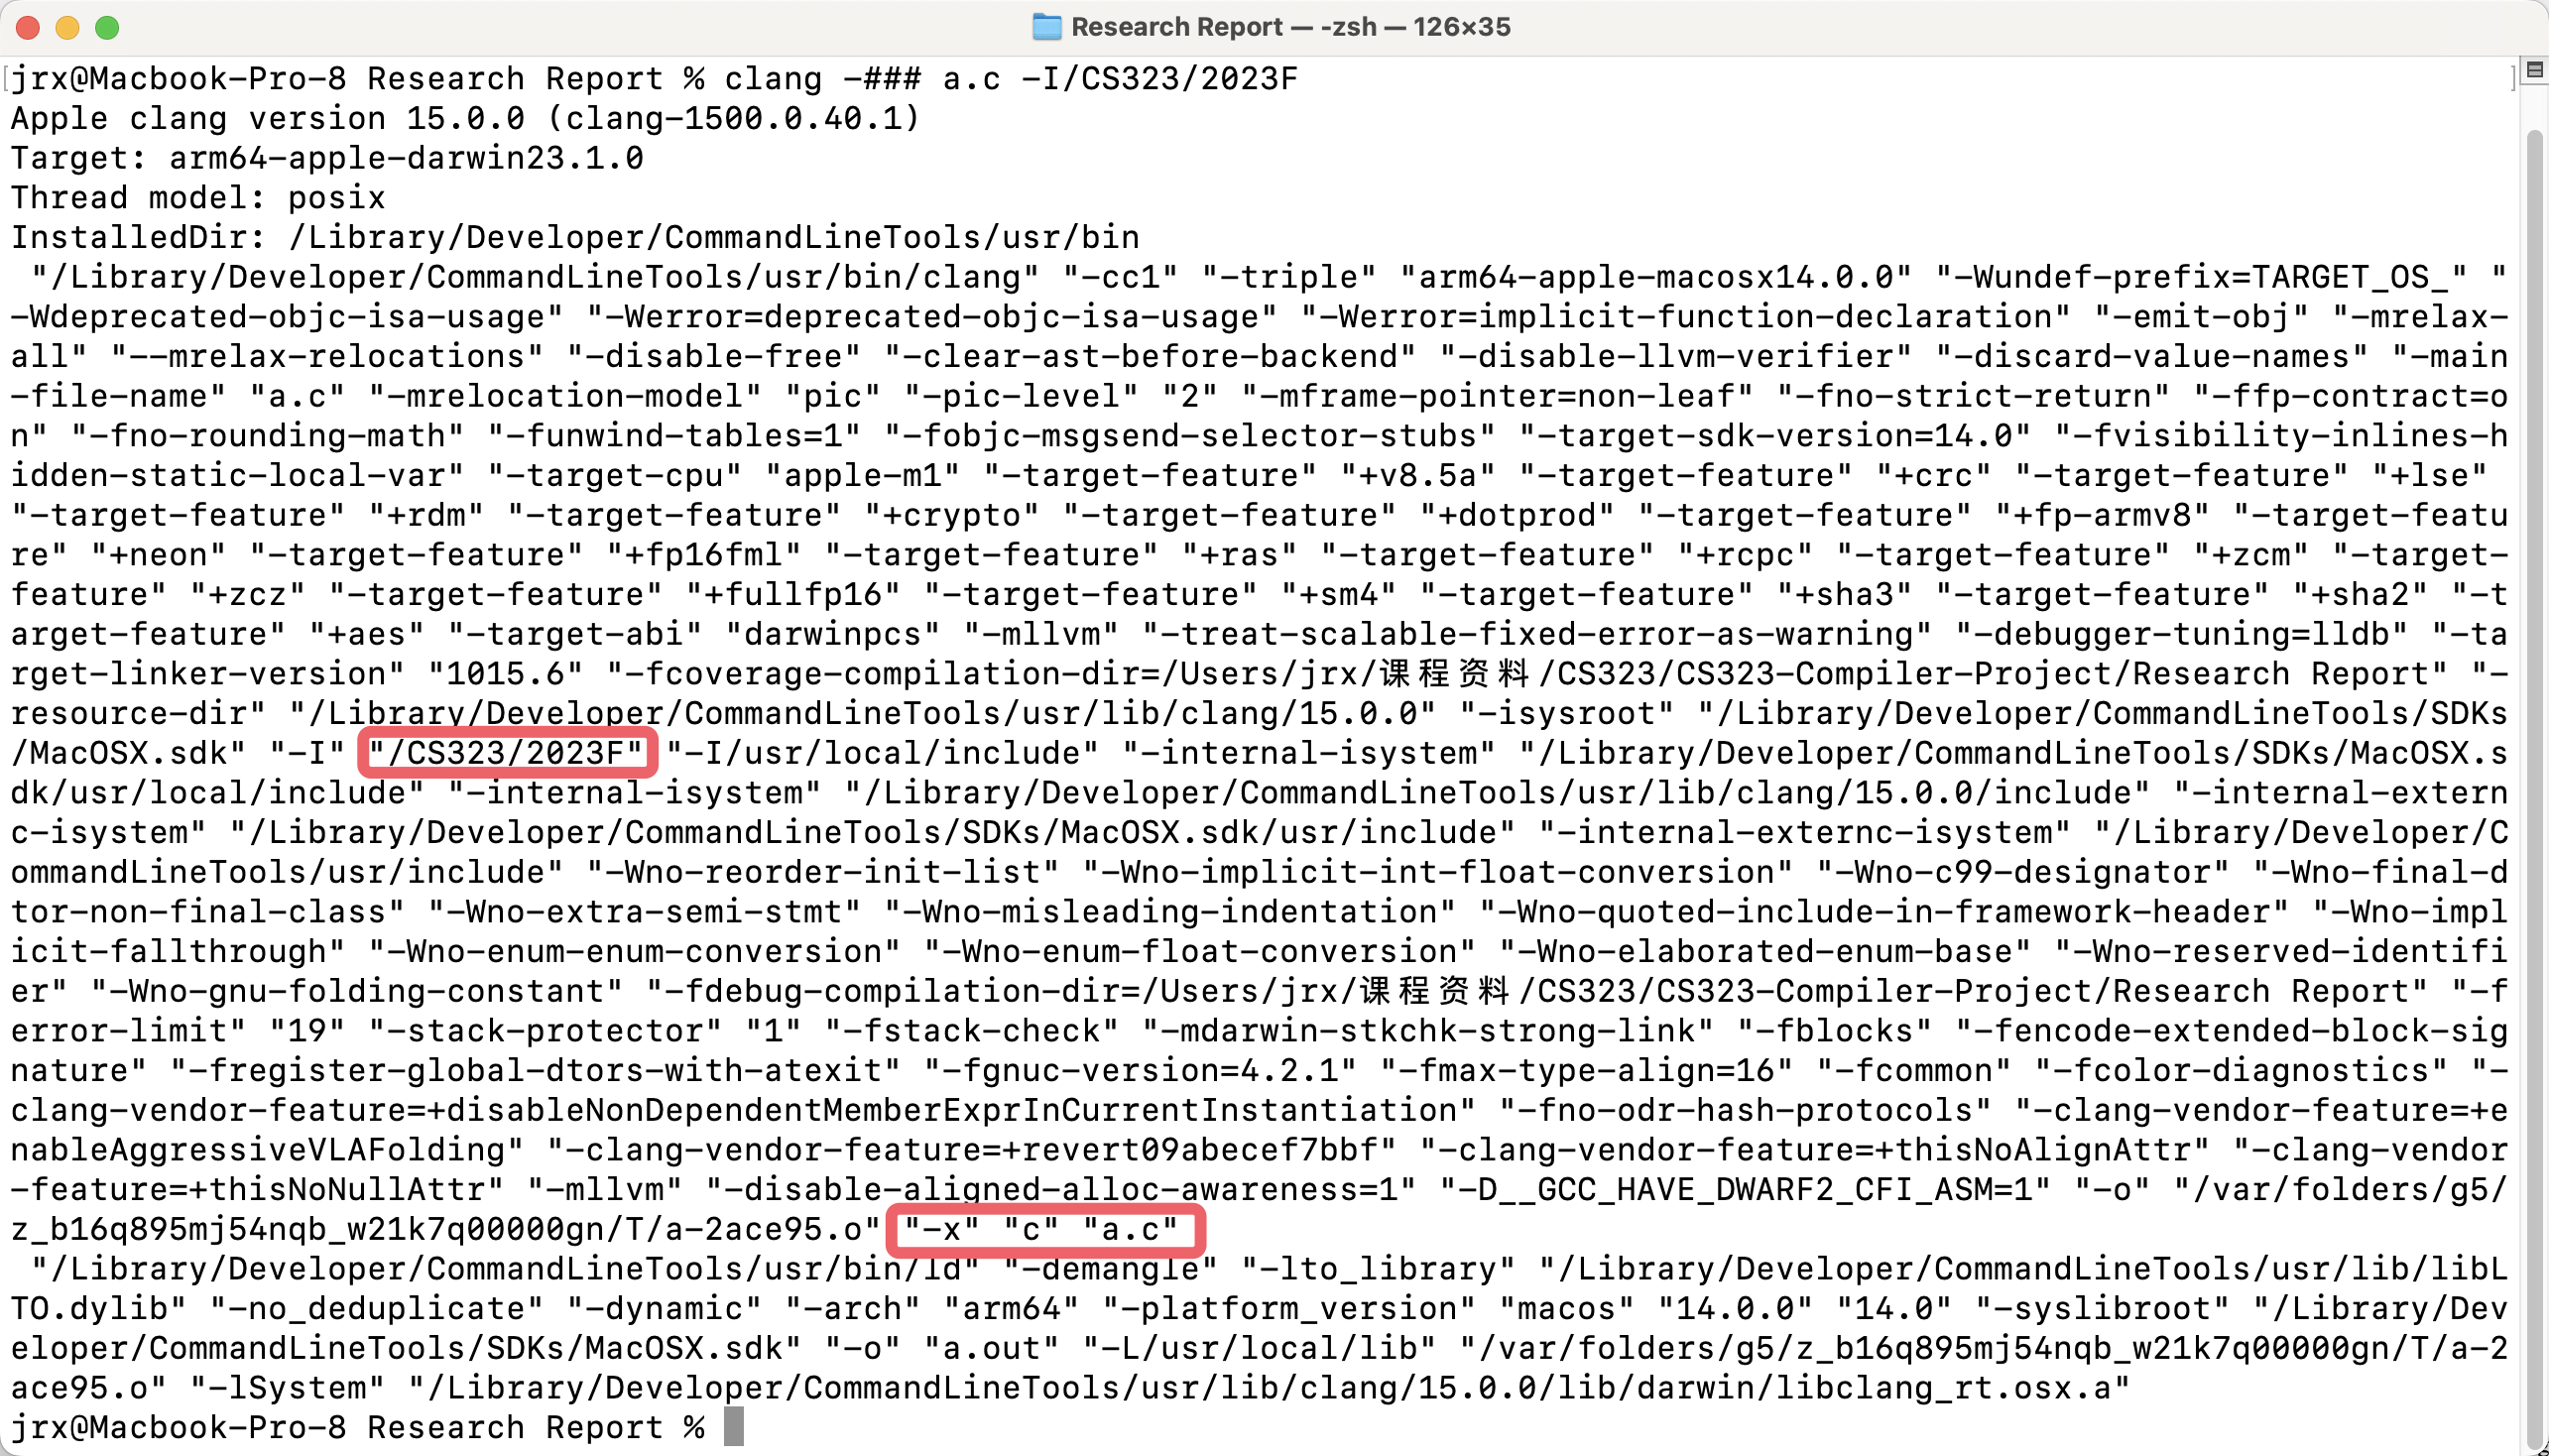
\includegraphics [width=1\linewidth]{pictures/DriverTerminal.png}
\caption{Parsing Output}
\label{fig17}
\end{figure}

It is noteworthy to focus on the two areas outlined by the red boxes in the diagram, as they represent the information passed to the compiler—specifically, the source file `a.c' that we intend to compile and the option `-I/CS323/2023F'.

In the first red box, we observe that the compiler splits `-I/CS323/2023F' into `-I' and `/CS323/2023F'. The `-I' option here is supported by Clang and, internally, is represented by OPT\_\_I, belonging to the Option class. Clang utilizes a Domain-Specific Language (DSL) specifically for handling options, storing them as .td files, processing them with table-gen to convert them into C++ code, and finally compiling them together with other C++ code. The value `/CS323/2023F' represents what -I receives as an argument. Here, we can see that the Driver layer handles this, parsing the `-I/CS323/2023F' we provide.

However, in comparison to `-I/CS323/2023F', the Driver processes the passed file a.c more extensively, indicated by `-x c a.c' in the second red box. The -x option in Clang specifies the compilation language required for the source code file. When Clang Driver recognizes a.c as a C language file, it appends the value c to the -x option, signifying the compilation of a C language file. How does Clang Driver know that this is a C language file? In essence, Clang Driver is rather simplistic; it determines this based on the file extension .c. Therefore, we can use -x c++ a.c to compile in C++ mode. If you have observed the compilation with clang and clang++, you would notice that clang++ is essentially clang, with defaults set for C++ compilation, hence all related options are geared towards C++. By the way, it's not a good idea using `clang a.cpp' or `clang x c++ a.cpp', which will cause several link errors. It's OK to use `clang a.cpp -lc++' instead, while clang++ is a better solution for cpp code.

Secondly, the role of the Pipeline is to construct different Compiler Actions based on specific compilation options.

Use `clang -ccc-print-phases a.c' to print the result after pipelining, which is shown in Figure 18.

\begin{figure}[htbp]
\centering
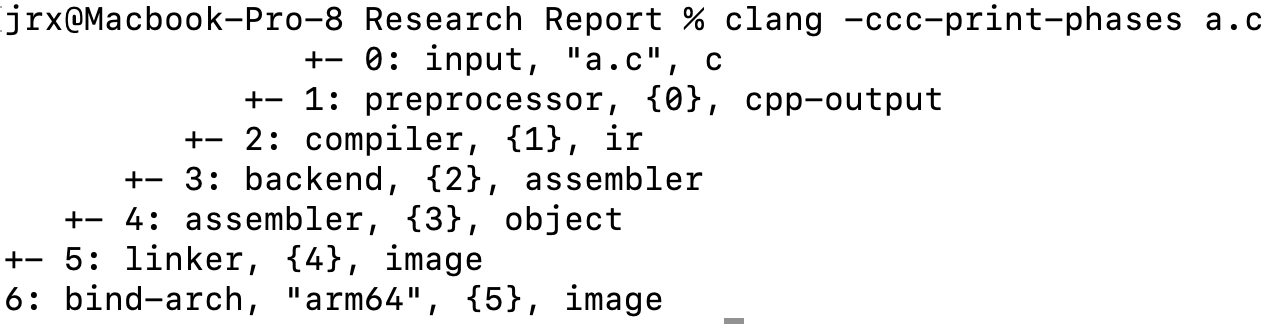
\includegraphics [width=0.9\linewidth]{pictures/Pipeline.png}
\caption{Pipeline Output}
\label{fig18}
\end{figure}

Here, we can observe a familiar process, such as using the preprocessor for preprocessing and then employing the compiler for compilation, and so on, with their respective outcomes. For instance, the preprocessed value is labeled as cpp-output. It's crucial to note that here, cpp doesn't refer to C++, but rather to the result of C language preprocessing. If it were C++, the output would be C++-cpp-output. This distinction is prone to confusion in the Clang codebase, where the former corresponds to .i files, and the latter to .ii files. Within the Clang Pipeline process, most actions correspond to actual occurrences, such as preprocessing and compilation. However, there are two distinctive actions: InputAction and BindArchAction. The former aids in facilitating actual actions, such as providing input files during preprocessing. BindArchAction is used to bind machine architecture with InputAction, as demonstrated in this example, where it is applied to Arm64. Because BindArchAction can bind input to different machine architectures, a common application is to concurrently create a library that supports both 32-bit and 64-bit architectures.

Thirdly, the role of Bind is to facilitate the selection of Tool and Filename.

When we create a series of Actions, Bind's role is to provide us with specific Tools to execute this sequence of actual operations. During actual execution, these operations take place as individual subprocesses. For example, if there is an Assemble Action, Assembler is responsible for performing the assembly work. But which Assembler to choose, the embedded one, GNU's or others, is determined by Bind. The selection of the Tool is handled by the ToolChain, where each architecture, platform, and operating system has its own ToolChain. Bind interacts with the ToolChain, and the ToolChain is responsible for choosing the specific Tool to complete a series of Actions. As for Filename, note that each Action may interact with another Action, and sometimes, one Action is the input for another. In such cases, we should focus on what form the input takes, inter-process communication, a pipeline, or a file, among other possibilities (actual Tools run as subprocesses, and various inter-process communication methods are detailed in operating system textbooks). If a file is used, Filename determines the kind of filename ultimately used.

Use `clang -ccc-print-bindings a.c' to print the result after binding, which is shown in Figure 19.

\begin{figure}[htbp]
\centering
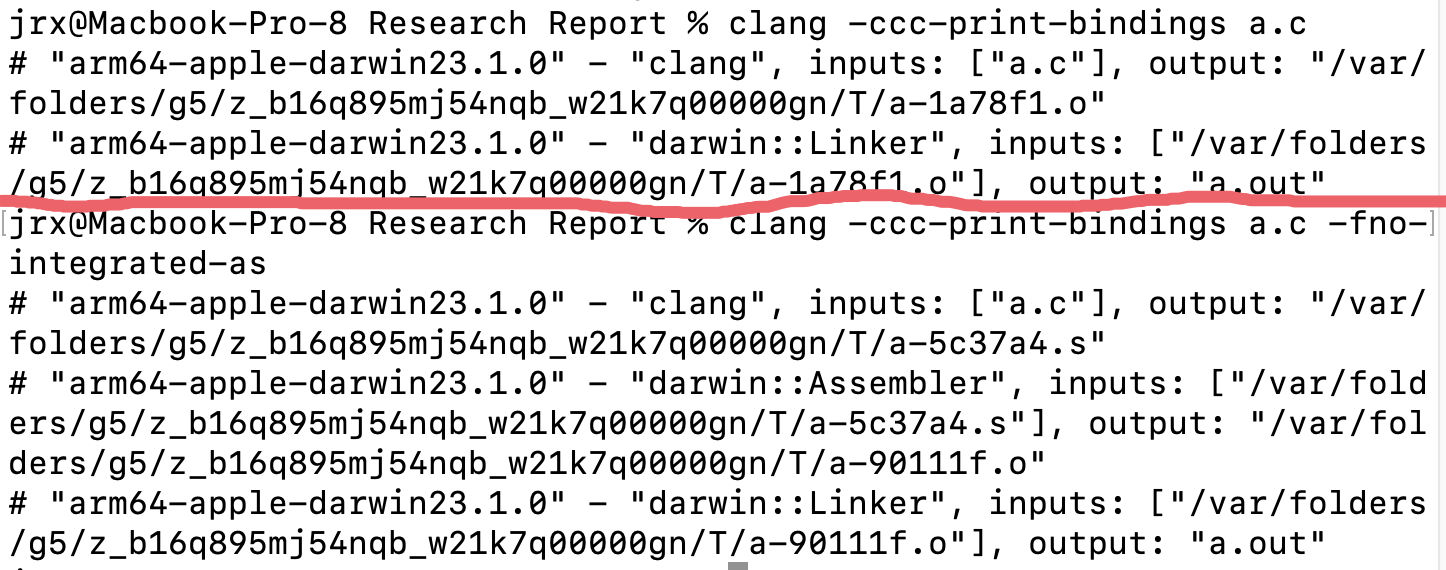
\includegraphics [width=0.9\linewidth]{pictures/Binding.png}
\caption{Bind Output}
\label{fig19}
\end{figure}

It can be observed that the compiler chosen is clang, and the linker selected is darwin::Linker. It seems that the assembly process and assembler are absent. In reality, on the Mac platform, Clang utilizes an integrated assembler, namely integrated-as. After generating LLVM IR, it calls the integrated assembler, directly producing the .o file. The advantage of this approach is the reduction of overhead associated with generating assembly files and invoking the target assembler. The option `-fno-integrated-as' can be used to instruct clang not to use the integrated assembler.

Fourthly, The role of Translate is to handle the translation of tool options and parameters.

This step involves mapping relevant parameters to tools on various platforms, closely integrated with the Bind process. Use `clang a.c -shared -v' to print the result of creating a dynamic library using the -shared option, which is shown in Figure 20. Note that the output may be different in other systems, for example, Ubuntu Linux.

\begin{figure}[htbp]
\centering
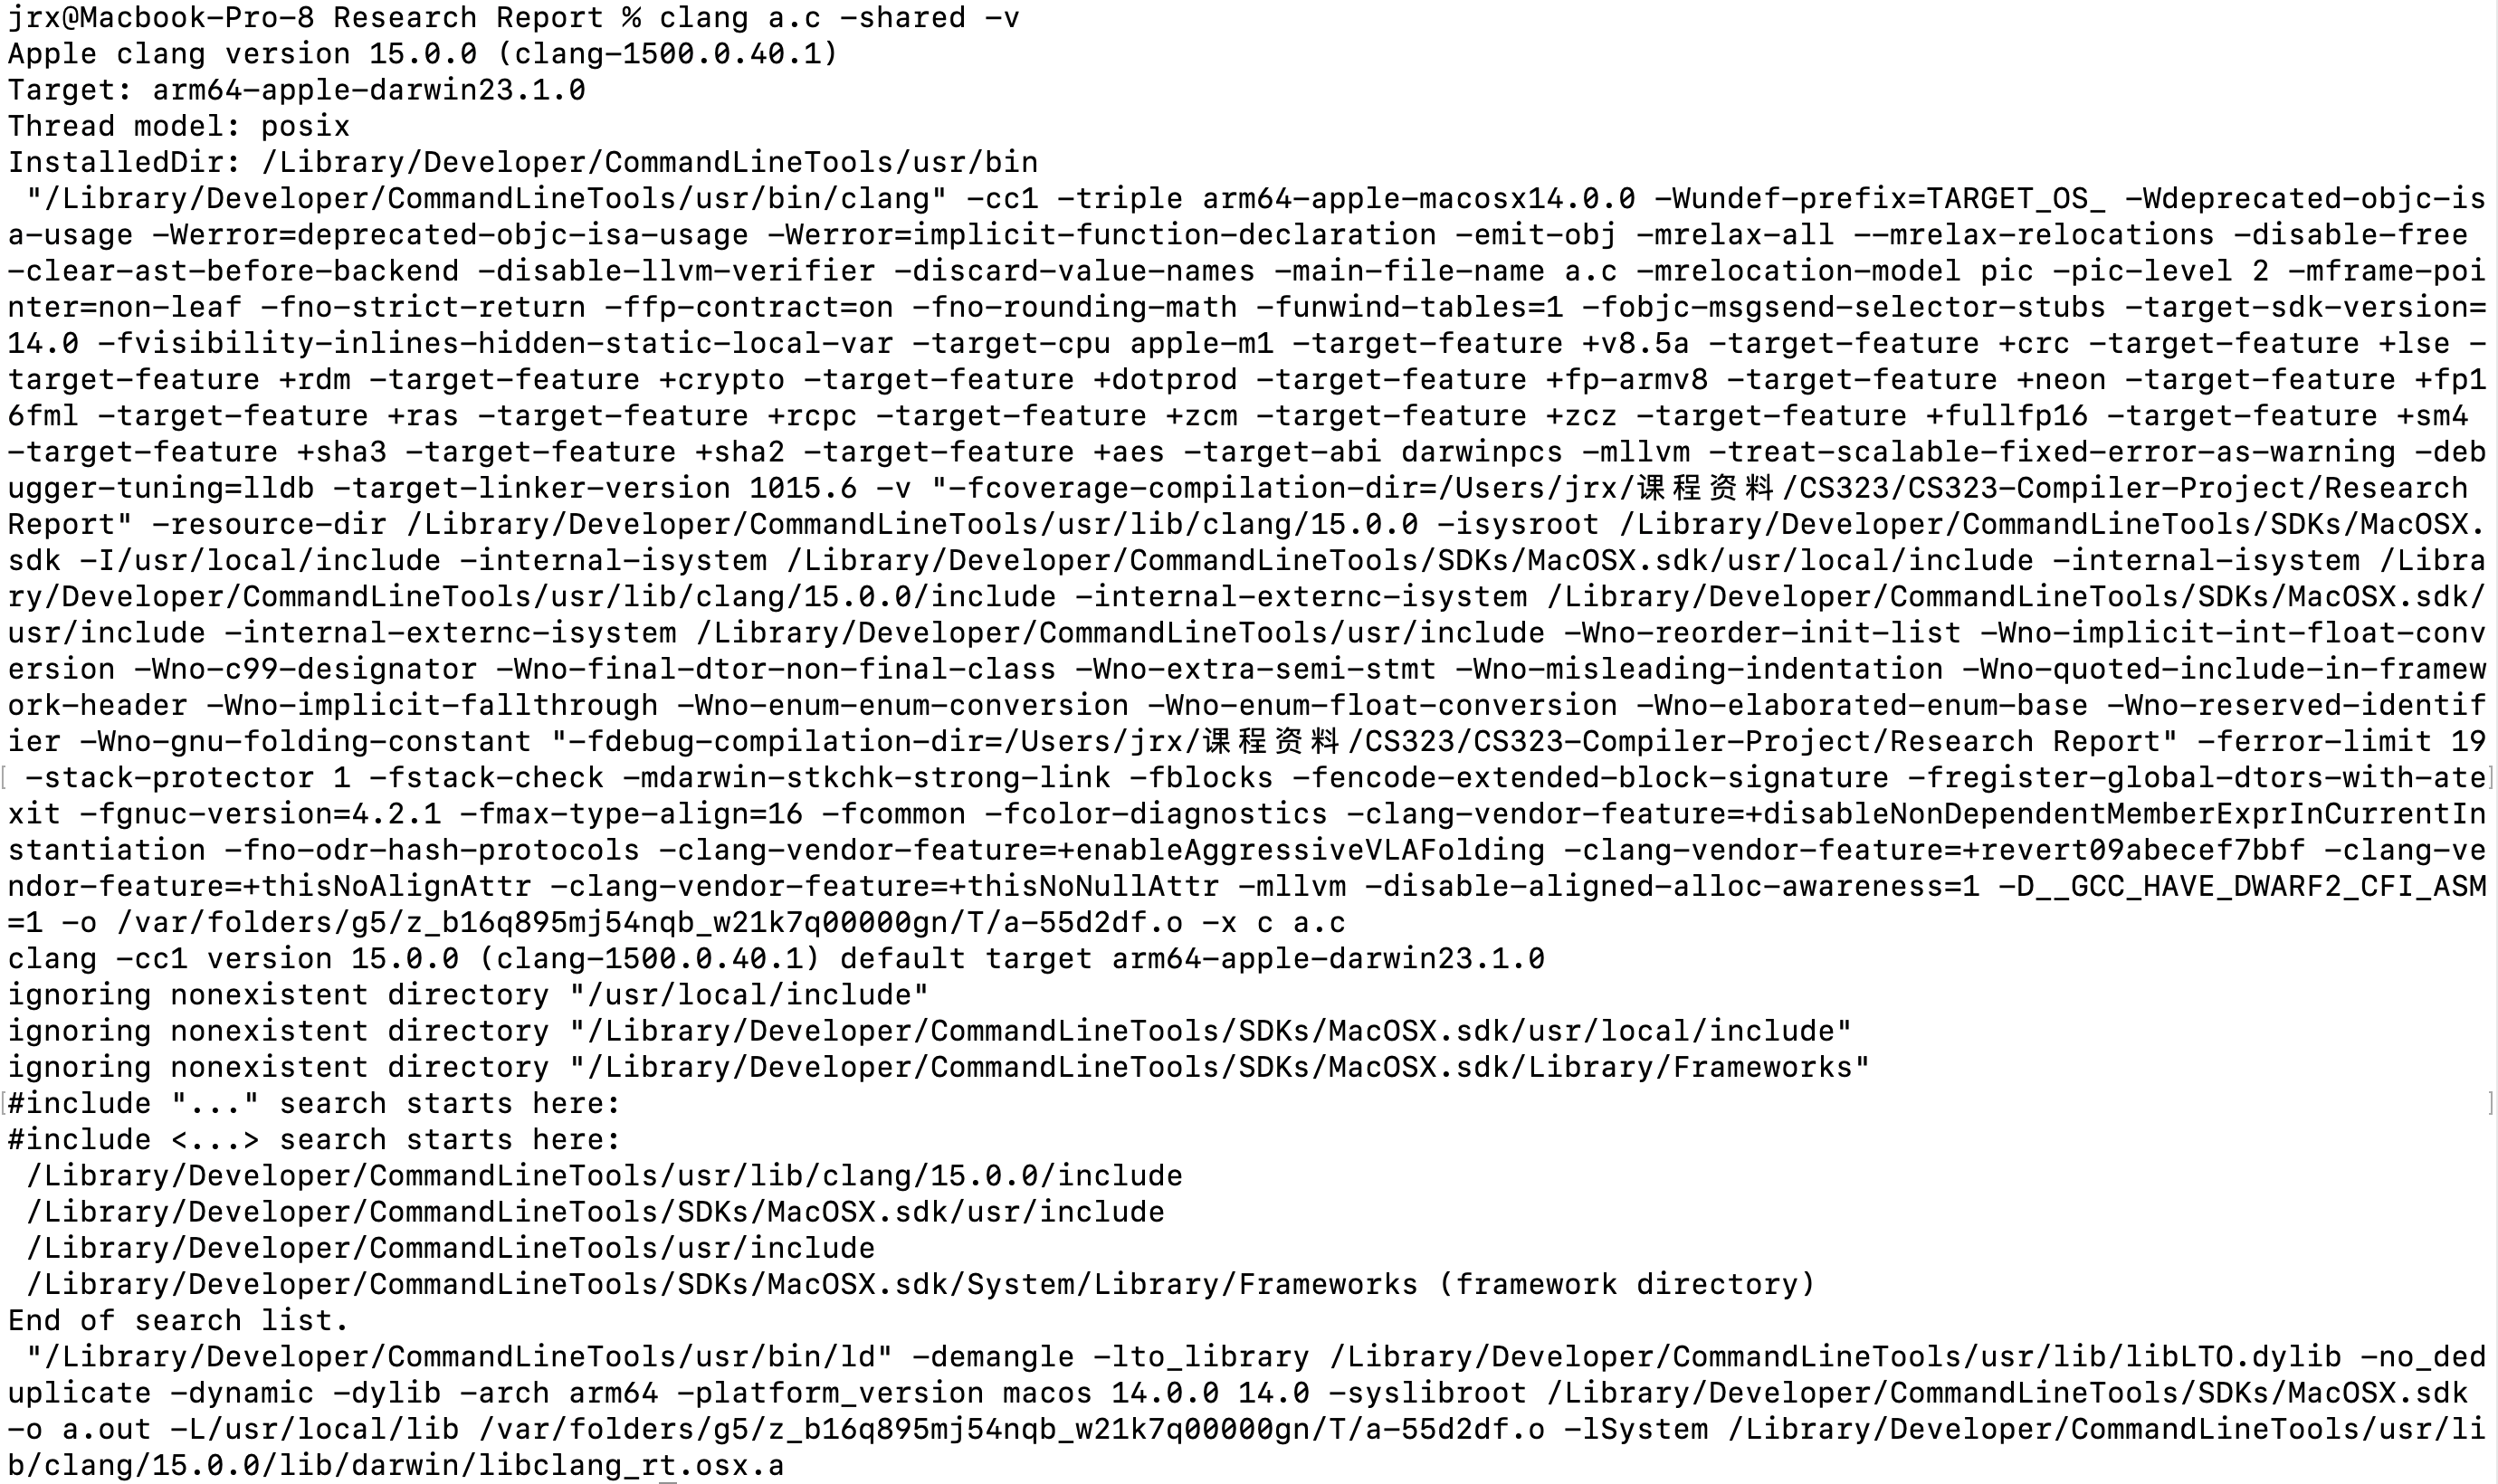
\includegraphics [width=1\linewidth]{pictures/Translate.png}
\caption{Translate Output}
\label{fig20}
\end{figure}

Fifthly, the role of Execute is to carry out the entire compilation process.

Use `clang a.c -ftime-report' to interact with it. Part of the output is shown in Figure 21.

\begin{figure}[htbp]
\centering
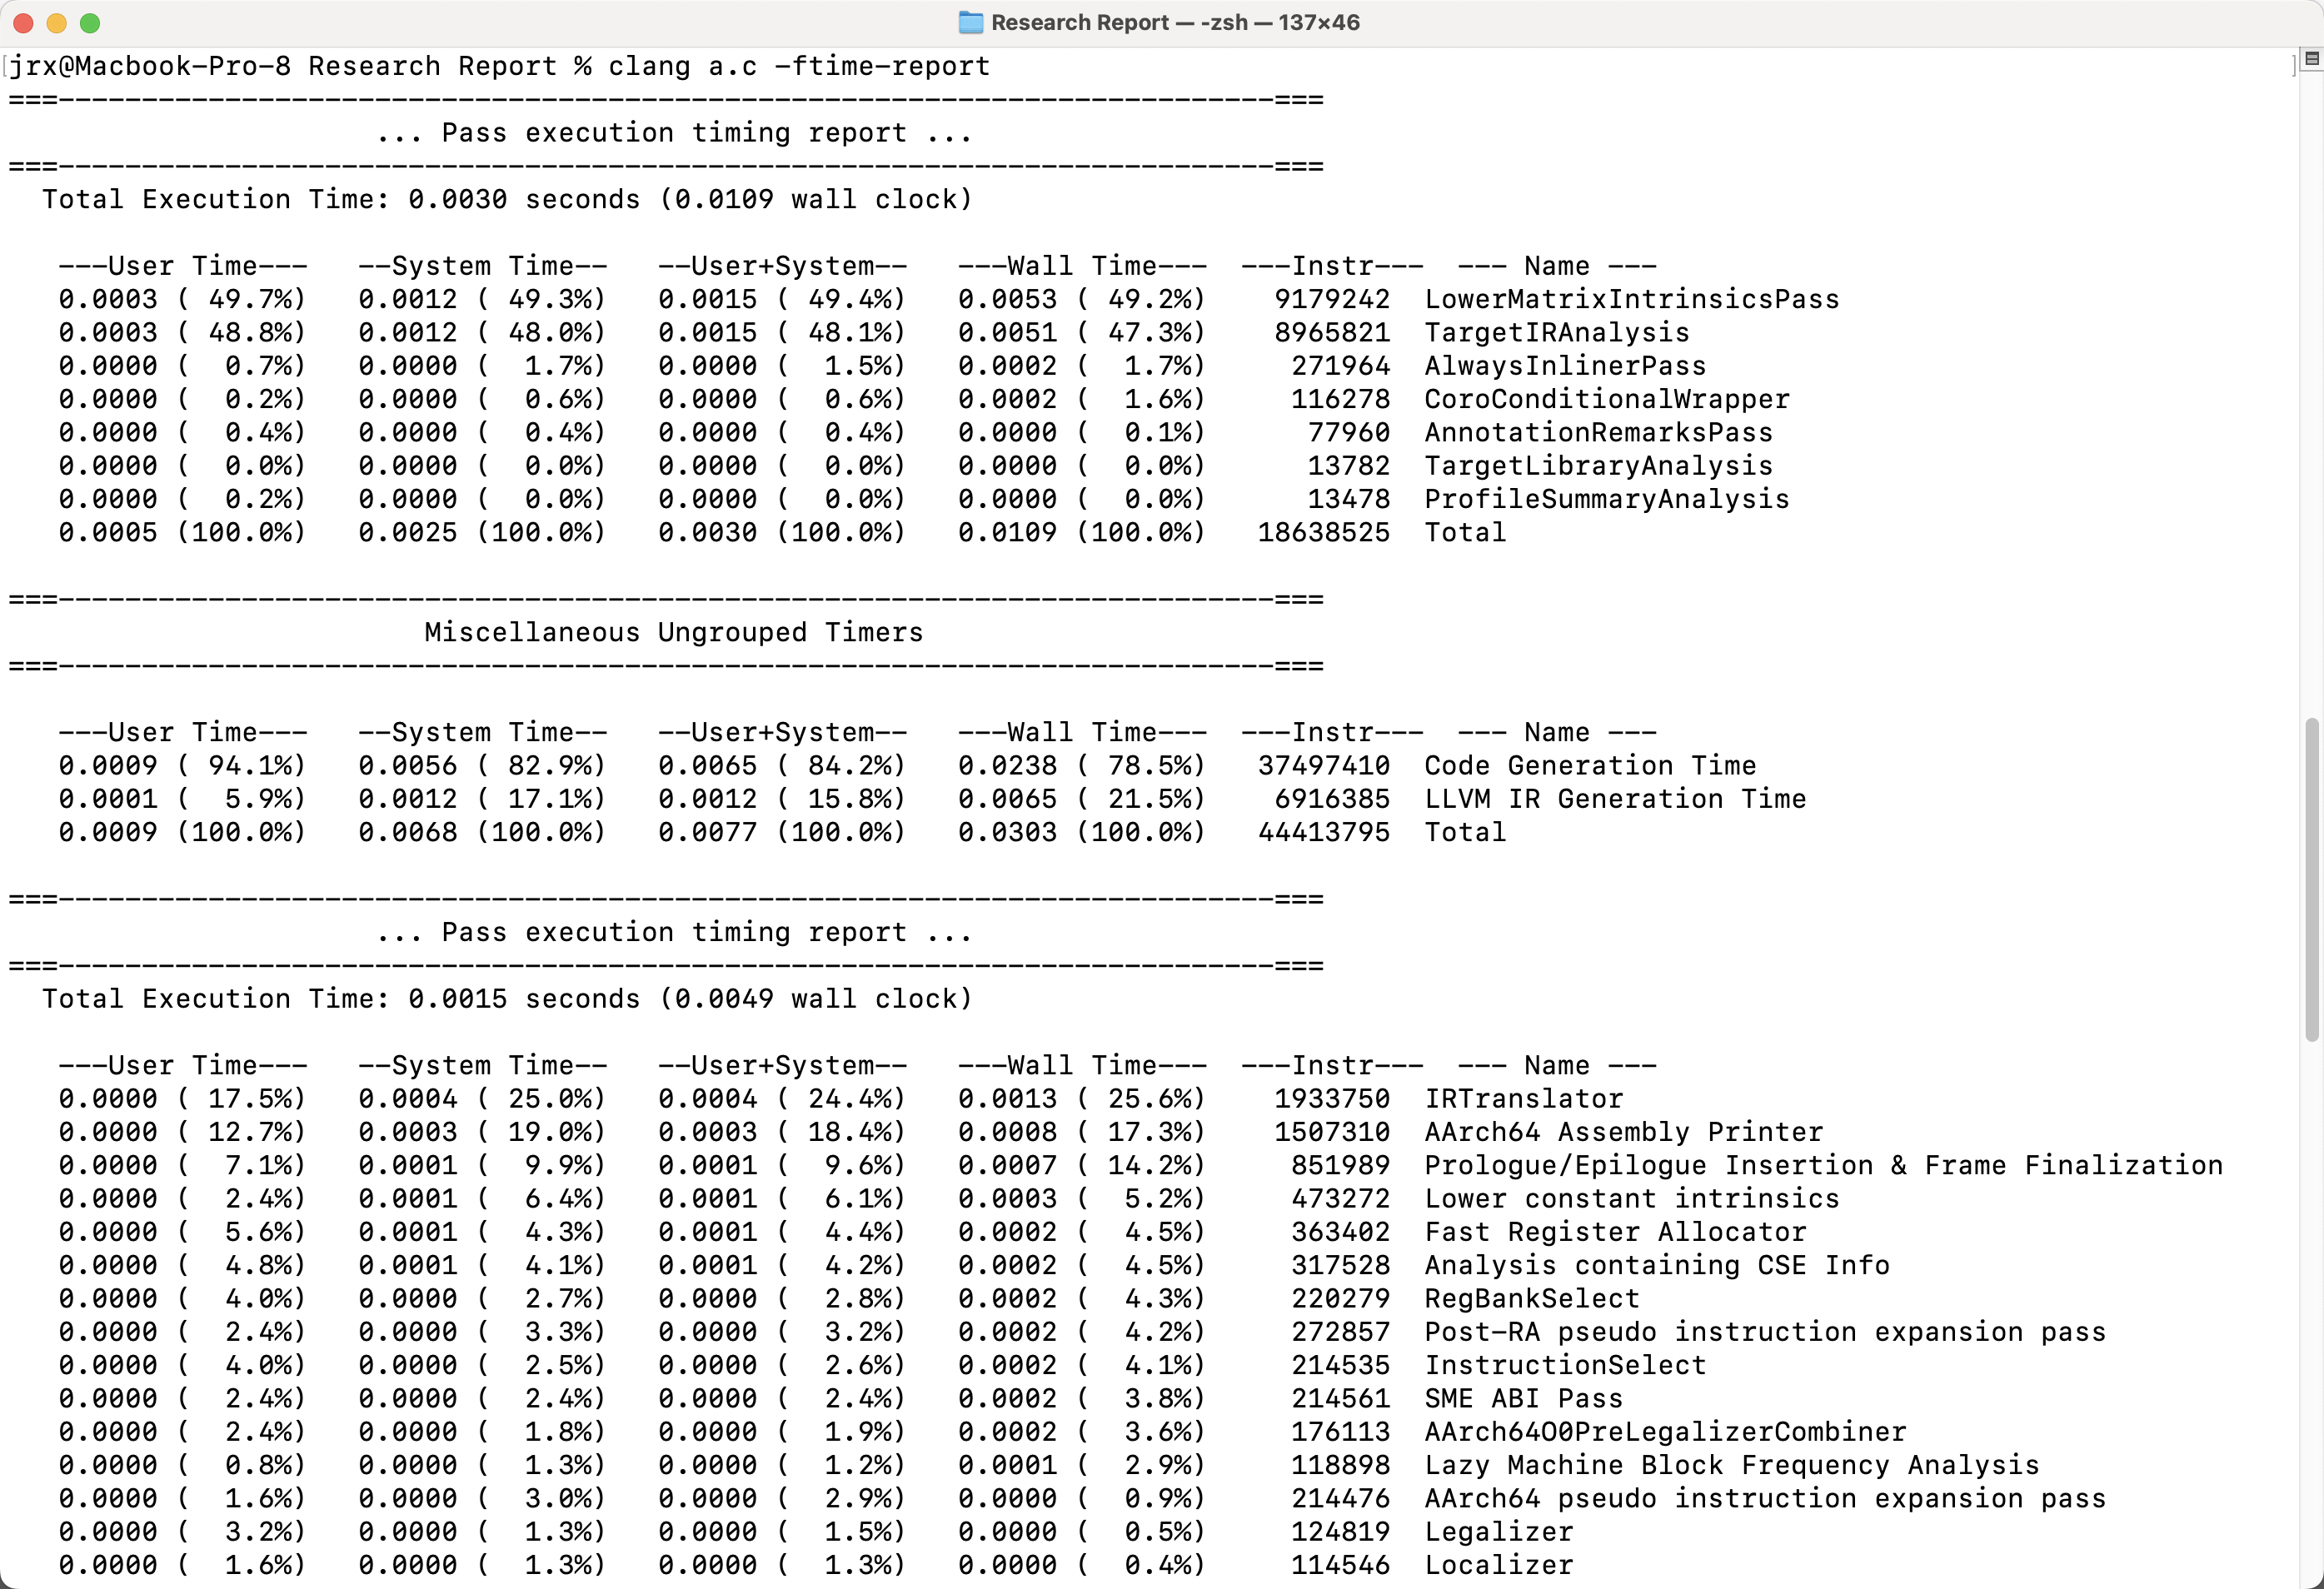
\includegraphics [width=1\linewidth]{pictures/Execute.png}
\caption{Execute Output}
\label{fig21}
\end{figure}

Additionally, clang-cl is an alternative command-line interface to Clang, designed for compatibility with the Visual C++ compiler, cl.exe. To enable clang-cl to find system headers, libraries, and the linker when run from the command-line, it should be executed inside a Visual Studio Native Tools Command Prompt or a regular Command Prompt where the environment has been set up using e.g. vcvarsall.bat. clang-cl can also be used from inside Visual Studio by selecting the LLVM Platform Toolset. The toolset is not part of the installer, but may be installed separately from the Visual Studio Marketplace. To use the toolset, select a project in Solution Explorer, open its Property Page (Alt+F7), and in the “General” section of “Configuration Properties” change “Platform Toolset” to LLVM. Doing so enables an additional Property Page for selecting the clang-cl executable to use for builds.\cite{b13}

\subsection{Summary of Clang/LLVM}

Clang/LLVM is a powerful and versatile compiler infrastructure that encompasses various functionalities crucial for modern software development.

Clang serves as a frontend compiler that supports a diverse range of programming languages, including C, C++, and Objective-C. It also provides robust and user-friendly diagnostics, offering detailed error and warning messages to aid developers in identifying and addressing code issues effectively.

The modular architecture of LLVM facilitates extensibility and ease of integration with new features and optimizations, making it adaptable to evolving compiler requirements. LLVM incorporates a sophisticated optimization framework that employs a wide range of techniques, including constant folding, loop optimizations, and inlining, to enhance the performance of generated code. Its code generation is target-independent, enabling developers to write portable code that can be optimized and executed on diverse hardware architectures.

Clang/LLVM stands as a versatile and efficient compiler infrastructure that not only delivers high-quality code generation but also offers a comprehensive set of tools and features to support modern software development practices.

\section{Comparison between GCC and Clang/LLVM}

The comparison between GCC and Clang/LLVM compilers involves assessing various aspects of their design, performance, and diagnostics. Both compilers are widely utilized in the software development community, each exhibiting strengths and considerations that merit examination.

\subsection{Design}

The GCC compiler takes source code as input and produces assembly code as output. This process is akin to the Clang phase in LLVM, including the IR linker and the assembly code generation part of the LLVM compiler. It's worth noting that Clang, in a streamlined process, doesn't generate assembly files, as it exclusively operates within an intermediate representation, treating the generation of assembly code and object files as parallel components.

The GCC assembler takes assembly code as input and generates object files as output. This functionality is analogous to LLVM's llvm-mc tool. While Clang, in its default workflow, bypasses this tool, it leverages the same libraries for descending and emitting assembly instructions.

The GCC linker, with object files as input, produces the final executable file. This corresponds to the Linker component in LLVM. Although LLVM has its linker (lld, released but still in development), the Clang driver currently invokes the system linker. Users have the flexibility to opt for the system linker or choose to use GCC's ld.

\subsection{Performance}

The goal is to evaluate the performance of the GCC and LLVM/clang compilers support for the RISC-V target and their ability to optimize for the architecture. The performance will be evaluated from executing CoreMark and Dhrystone which are both popular industry standard benchmarks for evaluating performance on embedded processors. They will be run on both the GCC and LLVM/clang compilers on different optimization levels and compared in performance per clock to the ARM architecture which is in comparison to RISC-V more mature yet the most similar widely used CPU architecture. As the result, -O2 and -O3 optimization levels on GCC performed very well, while LLVM/clang on the other hand crashed when trying to compile our CoreMark benchmark and on Dhrystone.\cite{b14}

\subsection{Diagnostics}

Compile the five .c files\cite{b15} in the `DiagnosticsPrograms' folder using both GCC and Clang compilers, and compare which compiler produces more reasonable error messages. Note that the version of GCC is gcc-13.2.0 while the version of Clang is clang-15.0.0. The results are shown in Figure 22 to Figure 24. The commands we use are `gcc -fsyntax-only -Wformat filename.c' and `clang -fsyntax-only -Wformat filename.c', respectively. For the first example, GCC detects that there are two errors, while Clang only detects one. For the second example, the two compilers give similar output. For the third example, GCC gives an exclusive note. Another 2 results are omitted due to the space limitation.

\begin{figure}[htbp]
\centering
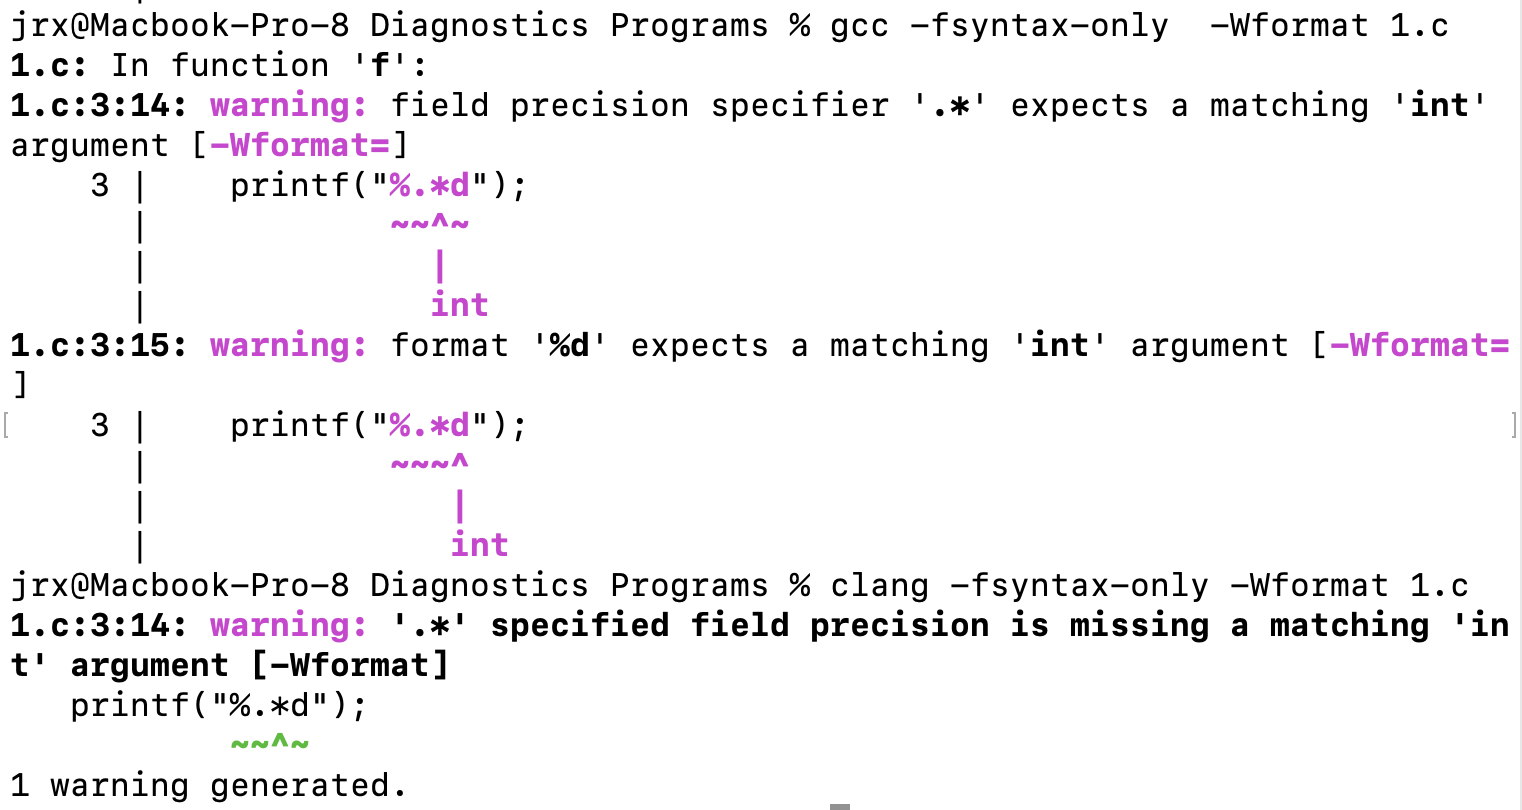
\includegraphics [width=0.8\linewidth]{Pictures/1.png}
\caption{Diagnostics Comparison 1}
\label{fig22}
\end{figure}

\begin{figure}[htbp]
\centering
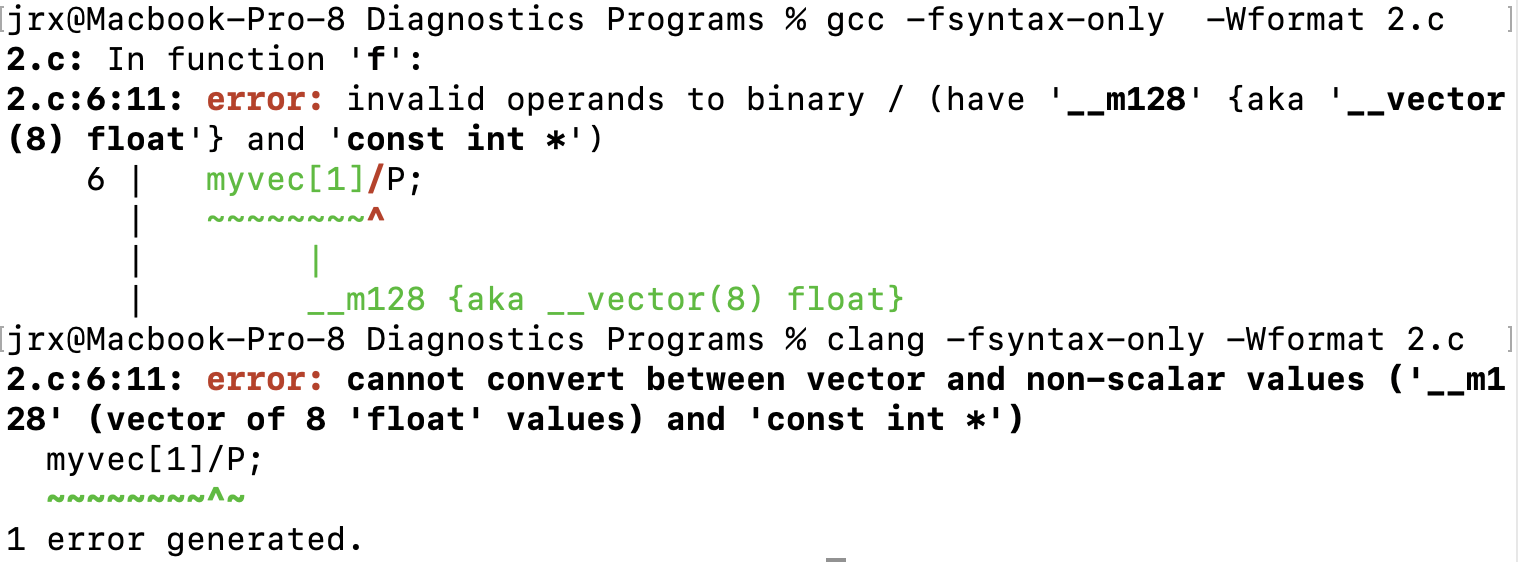
\includegraphics [width=0.8\linewidth]{Pictures/2.png}
\caption{Diagnostics Comparison 2}
\label{fig23}
\end{figure}

\begin{figure}[htbp]
\centering
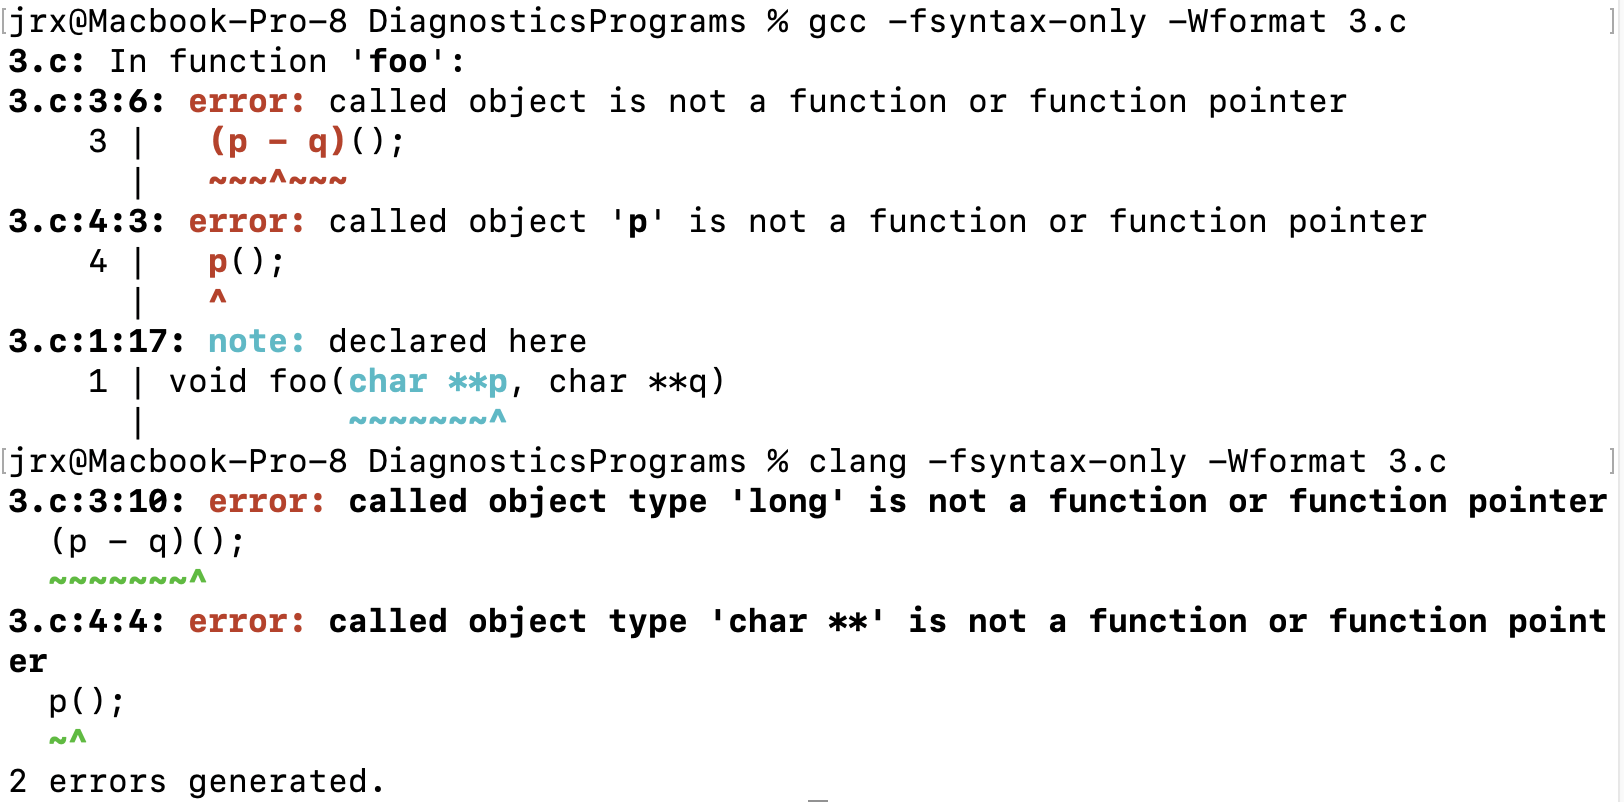
\includegraphics [width=0.8\linewidth]{Pictures/3.png}
\caption{Diagnostics Comparison 3}
\label{fig24}
\end{figure}

In brief, the compilation results of GCC and Clang are largely similar, with GCC providing more detailed error messages for certain examples. Additionally, GCC's error messages incorporate a greater use of color, enhancing their comprehensibility.

\subsection{Summary}

The choice between GCC and Clang/LLVM depends on specific project requirements and developer preferences. GCC's extensive language support and mature ecosystem appeal to many, while Clang/LLVM's modular architecture, superior diagnostics, and faster build times make it an attractive alternative, particularly in modern C++ development scenarios. Ultimately, the decision hinges on the unique needs and priorities of the development team and the characteristics of the project at hand.

\section{Conclusion}

In conclusion, our exploration and comparison of GCC, Clang, and LLVM have shed light on the diverse landscape of open-source compilers. These compilers, each with its unique strengths and characteristics, play pivotal roles in shaping the contemporary field of compiler technology.

Through our comparative analysis, we have unraveled architectural variances, optimization strategies, and distinct features, providing valuable insights for developers and the broader community. This research equips individuals with the knowledge to make informed decisions when selecting a compiler that aligns with their specific requirements. As the demand for efficient and high-performance compilers continues to evolve, the insights gained from this study will contribute to the ongoing advancements in compiler technology.


\begin{thebibliography}{00}

	\bibitem{b1} Novillo, D. (2006, September). GCC an architectural overview, current status, and future directions. In Proceedings of the linux symposium (Vol. 2, p. 185).
	\bibitem{b2} GNU Compiler Collection. (2017). Optimize Options. GNU Compiler Collection Documentation. Retrieved from https://gcc.gnu.org/onlinedocs/gcc-7.2.0/gcc/Optimize-Options.html
	\bibitem{b3} Bharatiya, P. (2023, November 1). Maximizing C++ Program Performance: A Comprehensive Guide to GCC Compiler Optimization. Data Intelligence. Retrieved from https://data-intelligence.hashnode.dev/maximizing-c-program-performance-a-comprehensive-guide-to-gcc-compiler-optimization
	\bibitem{b4} Jones, M. T. (2005). Optimization in GCC. Linux journal, 2005(131), 11.
	\bibitem{b5} Qingyang CHEN. (2023, November 9). Retrieved from https://zhuanlan.zhihu.com/p/337756824
	\bibitem{b6} GNU Compiler Collection. Vector Extensions. GNU Compiler Collection Documentation. Retrieved from https://gcc.gnu.org/onlinedocs/gcc/Vector-Extensions.html
	\bibitem{b7} Xiaowei, W., Kuixing, W., Quansheng, Y. (2012). Research and Development of Compiler Based on GCC. Recent Advances in Computer Science and Information Engineering: Volume 3, 809-814.
	\bibitem{b8} P2Tree. (2019). https://blog.csdn.net/SiberiaBear/article/details/103111028
	\bibitem{b9} Blue. (2016). https://zhuanlan.zhihu.com/p/21889573
	\bibitem{b10} LLVM. (2023). GlobalValue Class Reference. Retrieved from https://llvm.org/doxygen/classllvm\_1\_1GlobalValue.html
	\bibitem{b11} LLVM. (2023). LLVM Language Reference. Retrieved from https://llvm.org/docs/LangRef.html
	\bibitem{b12} Blue. (2017). https://zhuanlan.zhihu.com/p/22974869
	\bibitem{b13} LLVM Project. (2023). Clang User's Manual. LLVM. https://clang.llvm.org/docs/UsersManual.html\#clang-cl
	\bibitem{b14} Bjäreholt, J. (2017). RISC-V Compiler Performance: A Comparison between GCC and LLVM/clang.
	\bibitem{b15} GNU Project. (n.d.). ClangDiagnosticsComparison - GCC Wiki. GCC - GNU Project - Free Software Foundation (FSF). https://gcc.gnu.org/wiki/ClangDiagnosticsComparison


\end{thebibliography}

\vspace{12pt}
\end{document}
